\chapter{最优运输}
\label{chap:optimal-transport}

直线上的三个位置$0,1,2$各有一份质量，分别是$0.5$、$0.3$、$0.2$；我们想把它们重新摆成$0.2$、$0.3$、$0.5$的样子。搬动一份质量的代价是质量乘以搬运距离的平方。怎样搬最省？两份质量表都是概率分布，每一种搬法都是一张行和、列和固定的非负表，也就是两个分布的一个耦合。第~\ref{chap:distribution-comparison}章用耦合的最小成本定义了Wasserstein距离，那里只需要这个最小值；本章把“怎样达到它”本身作为问题：给定两个边缘分布和一个成本，在全部耦合中找成本最低的那一个。

这个问题有三层。第一层是问题本身是否有解：耦合允许把一个点的质量拆开送往几处，要求“一个点只去一处”的运输映射则可能根本不存在；最低成本是否真被某个耦合取到，也要看成本和分布满足什么条件。第二层是怎样确认手里的方案已经最优：每个可行方案都给出最低成本的一个上界，对偶问题给出下界，两者相等时方案就被证实。第三层是怎样把它算出来：实数轴上的顺序、有限点上的线性规划、高斯分布的二次结构各自给出可计算的形式；一般的有限问题还可以加上熵正则化，用简单的交替缩放求近似解。

最后两节把最优耦合当作工具，构造新的分布。沿最优耦合把每份质量匀速推向目的地，得到连接两个分布的一条路径；对多个分布按权重求总运输成本最小的分布，得到它们的Wasserstein重心。这两种构造都移动质量的位置，与按权重混合两个分布完全不同。

本章回用第~\ref{chap:distribution-comparison}章的耦合、Wasserstein距离与有限支撑的Kantorovich--Rubinstein对偶，第~\ref{chap:weak-convergence-of-distributions}章的胎紧与弱收敛子列，第~\ref{chap:random-variables}章的分位数，以及线性规划的对偶理论。全章贯穿开头的三点例子。

\section{运输问题}
\label{sec:ot-problem}

先把章首的例子写成表。源位置$x=0,1,2$上的质量是
\[
 \bm{a}=(0.5,\ 0.3,\ 0.2),
\]
目标位置$y=0,1,2$上需要的质量是
\[
 \bm{b}=(0.2,\ 0.3,\ 0.5),
\]
把一份质量$m$从$x$搬到$y$的代价是$m\,(x-y)^{2}$，记成本矩阵$\bm{C}$，元素$c_{i,j}=(i-j)^{2}$（下标从$0$起）。一个搬运方案说清从每个$x_i$搬多少到每个$y_j$，即一个$3\times3$的非负表$\bm{\pi}$；从$x_i$出发的总量要等于$a_i$，到达$y_j$的总量要等于$b_j$，也就是行和为$\bm{a}$、列和为$\bm{b}$。

图~\ref{fig:ot-supply-arrows}画出两种自然的搬法。(a)把$0$处多出的$0.3$搬到$1$，同时把$1$处原有的$0.3$搬到$2$，每份质量只走一格；(b)让$1$处不动，把$0$处多出的$0.3$直接搬到$2$。若成本只按距离一次方计，两者都是$0.6$，这是第~\ref{chap:distribution-comparison}章见过的现象；按平方成本计，(a)的花费是$0.3\cdot1+0.3\cdot1=0.6$，(b)是$0.3\cdot4=1.2$。

\begin{BookInlineFigure}
 \centering
 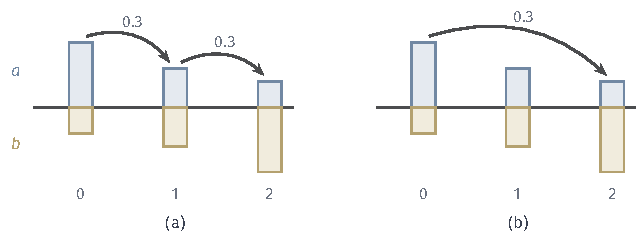
\includegraphics[width=108mm]{figures/07-probability/07-distribution-optimization/tikz/ot-supply-arrows/figure.pdf}
 \caption{全章例子：蓝柱向上是源质量$\bm{a}=(0.5,0.3,0.2)$，黄柱向下是目标质量$\bm{b}=(0.2,0.3,0.5)$，位置为$0,1,2$；箭头上的数是搬运的质量，未画箭头的质量留在原地。(a)逐格搬运，平方成本$0.6$。(b)跳格搬运，平方成本$1.2$。}
 \label{fig:ot-supply-arrows}
\end{BookInlineFigure}

还有许多别的搬法。最“不动脑筋”的是独立搬运：从$x_i$出发的质量按$\bm{b}$的比例分给各个目标，$\pi_{i,j}=a_ib_j$。图~\ref{fig:ot-plan-tables}把三个方案写成表，它们的行和、列和完全相同，平方成本却分别是$1.58$、$1.2$和$0.6$。同一对边缘分布，因质量配对方式不同而产生不同成本；本章的问题就是在全部配对方式中找成本最低的那一个。

\begin{BookInlineFigure}
 \centering
 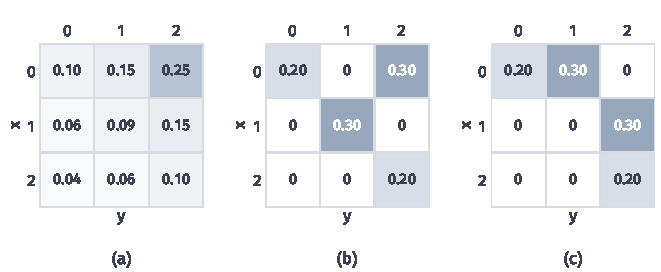
\includegraphics[width=112mm]{figures/07-probability/07-distribution-optimization/matplotlib/ot-plan-tables/figure.pdf}
 \caption{全章例子的三个运输方案，行是源位置$x$，列是目标位置$y$，颜色越深质量越大。三张表的行和都是$\bm{a}$，列和都是$\bm{b}$。(a)独立方案$\pi_{i,j}=a_ib_j$，平方成本$1.58$。(b)跳格搬运，平方成本$1.2$。(c)逐格搬运，平方成本$0.6$。}
 \label{fig:ot-plan-tables}
\end{BookInlineFigure}

这里有三个不同的问题。其一，在全部满足行列约束的方案中优化，允许把一个位置的质量拆开送往几处，这是耦合上的优化。其二，要求每个源位置的质量整体送到一个目标位置，这是运输映射上的优化，可行的方案少得多，甚至可能没有。其三，确认最低成本确实被某个方案取到，而不只是一个无法达到的下确界。下面三小节依次处理。把最低成本当作分布之间的距离时，它的对称性、三角不等式以及与弱收敛的关系已在第~\ref{chap:distribution-comparison}章讨论，本章不再重复。

\subsection{固定边缘的耦合}
\label{sec:ot-couplings}

有限情形的方案是一张非负表。设源有$m$个位置，质量向量$\bm{a}\in\mathbb{R}^{m}$；目标有$n$个位置，质量向量$\bm{b}\in\mathbb{R}^{n}$；两者都非负且总和为$1$。可行方案的全体是
\begin{equation}
 U(\bm{a},\bm{b})=\bigl\{\bm{\pi}\in\mathbb{R}^{m\times n}:\ \bm{\pi}\geq0,\ \bm{\pi}\bm{1}=\bm{a},\ \bm{\pi}^{\top}\bm{1}=\bm{b}\bigr\},
 \label{eq:ot-transport-polytope}
\end{equation}
其中$\bm{\pi}\geq0$指每个元素非负，$\bm{1}$是全一向量。它由有限个线性等式和不等式刻画，是一个有界的凸多面体，称为\term{运输多面体}（transport polytope）。总成本是线性函数
\[
 \langle\bm{C},\bm{\pi}\rangle=\sum_{i,j}c_{i,j}\pi_{i,j} .
\]

把$\bm{\pi}$看成取值于$\{x_i\}\times\{y_j\}$的随机向量$(X,Y)$的联合概率表，行和、列和约束就是“$X$的边缘为$\bm{a}$，$Y$的边缘为$\bm{b}$”，总成本就是$\mathbb{E}[c(X,Y)]$。这正是第~\ref{chap:distribution-comparison}章的耦合：$\mathcal{X}$上的分布$\mu$与$\mathcal{Y}$上的分布$\nu$的耦合是$\mathcal{X}\times\mathcal{Y}$上边缘分别为$\mu,\nu$的分布，全体记作$\Pi(\mu,\nu)$。有限情形$\Pi(\mu,\nu)$与$U(\bm{a},\bm{b})$一一对应。一般情形不再有表，但问题的写法不变。

\begin{definition}[最优运输问题]
\label{def:ot-problem}
设$\mu,\nu$分别是$\mathcal{X},\mathcal{Y}$上的概率分布，$c:\mathcal{X}\times\mathcal{Y}\to[0,\infty]$可测。对耦合$\pi\in\Pi(\mu,\nu)$，称$\int c\,\mathrm{d}\pi$为它的运输成本。称
\begin{equation}
 \operatorname{OT}_c(\mu,\nu)=\inf_{\pi\in\Pi(\mu,\nu)}\int_{\mathcal{X}\times\mathcal{Y}}c(x,y)\,\pi(\mathrm{d}x,\mathrm{d}y)
 \label{eq:ot-kantorovich}
\end{equation}
为\term{最优运输问题}（optimal transport problem）的最优值。耦合也称为\term{运输方案}（transport plan）；达到下确界的耦合称为\term{最优耦合}（optimal coupling）。
\end{definition}

定义要求成本非负，是为了让每个耦合的成本都有意义：非负可测函数的积分总有定义，取值在$[0,\infty]$中，不会出现$\infty-\infty$。若成本有界或下方被可积函数控制，也可以同样处理，但本章只用非负成本。取$\mathcal{X}=\mathcal{Y}$为度量空间、$c=d^{p}$时，$\operatorname{OT}_c^{1/p}$就是第~\ref{chap:distribution-comparison}章的$W_p$。

可行集合从不为空：乘积分布$\mu\otimes\nu$总是一个耦合，它对应“让$X$与$Y$独立”，在有限情形就是图~\ref{fig:ot-plan-tables}(a)的独立方案。但可行不等于有有限成本的方案。取$\mu=\delta_0$，$\nu$为标准Cauchy分布，$c(x,y)=(x-y)^{2}$。$\mu$只有一个点，任何耦合的第一个分量都恒为$0$，所以$\Pi(\mu,\nu)$只有$\delta_0\otimes\nu$一个元素。Cauchy密度与$1/(1+y^{2})$成正比，乘以$y^{2}$后在远处趋于正常数，所以这个唯一耦合的成本是
\[
 \int y^{2}\,\nu(\mathrm{d}y)=\infty .
\]
最优值是$\infty$，问题虽然可行，却给不出任何有用的比较。对$c=\lvert x-y\rvert^{p}$，只要两个分布都有有限$p$阶矩，第~\ref{chap:distribution-comparison}章的估计就说明独立耦合的成本有限；本章讨论的具体问题都满足这类条件。

\subsection{运输映射}
\label{sec:ot-maps}

耦合允许把一个点的质量拆开。如果规定每个源点的质量必须整体送到同一个目标点，方案就由一个函数$T:\mathcal{X}\to\mathcal{Y}$描述：$x$处的质量全部送到$T(x)$。目标处收到的质量分布是$\mu$在$T$下的推前$T_\#\mu$，即$T_\#\mu(B)=\mu(T^{-1}(B))$，推前测度的一般性质可参考\BookChapterRef{chap:pushforward-measures}{卷四第9章“推前测度”}。满足
\begin{equation}
 T_\#\mu=\nu
 \label{eq:ot-transport-map}
\end{equation}
的可测映射称为从$\mu$到$\nu$的\term{运输映射}（transport map）。在映射中优化成本$\int c(x,T(x))\,\mu(\mathrm{d}x)$称为\term{Monge问题}（Monge problem）。

映射是耦合的特例。设$X\sim\mu$，令$Y=T(X)$，则$(X,Y)$的联合分布是
\[
 \pi_T=(\mathrm{id},T)_\#\mu ,
\]
它把全部质量放在$T$的图像$\{(x,T(x))\}$上。它的第一个边缘是$\mu$，第二个边缘是$T_\#\mu=\nu$，所以$\pi_T\in\Pi(\mu,\nu)$，并且$\int c\,\mathrm{d}\pi_T=\mathbb{E}[c(X,T(X))]$。于是Monge问题的下确界不小于$\operatorname{OT}_c(\mu,\nu)$：映射能做的，耦合都能做。

反过来不成立，而且差别可能是根本性的。取$\mu=\delta_0$，$\nu=\tfrac12\delta_{-1}+\tfrac12\delta_1$。任何映射都把$\delta_0$推成单点分布$\delta_{T(0)}$，不可能等于有两个原子的$\nu$，所以映射问题连可行解都没有。耦合问题却有唯一的可行解$\delta_0\otimes\nu$：$0$处的单位质量一分为二，各送一半到$\pm1$，见图~\ref{fig:ot-split-map}(a)。

\begin{BookInlineFigure}
 \centering
 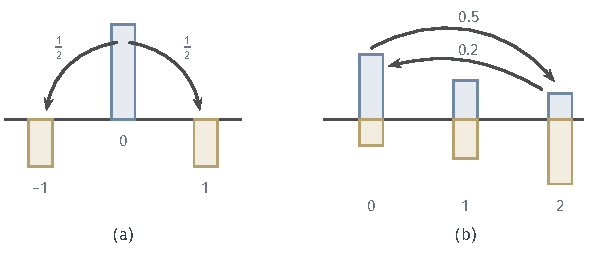
\includegraphics[width=100mm]{figures/07-probability/07-distribution-optimization/tikz/ot-split-map/figure.pdf}
 \caption{映射与耦合。(a)$\delta_0$到$\tfrac12\delta_{-1}+\tfrac12\delta_1$：唯一的耦合把单位质量拆成两半，没有映射能做到。(b)全章例子中唯一的运输映射$T(0)=2$，$T(1)=1$，$T(2)=0$，平方成本$2.8$。}
 \label{fig:ot-split-map}
\end{BookInlineFigure}

全章例子中映射是存在的，但选择极少。$T$把每个源位置的整份质量送到一个目标位置，所以每个$b_j$必须等于若干个$a_i$之和。$b_0=0.2$只能由$a_2=0.2$凑成，$b_1=0.3$只能由$a_1$凑成，剩下$a_0=0.5$正好是$b_2$，于是唯一的映射是$T(0)=2$，$T(1)=1$，$T(2)=0$，平方成本$0.5\cdot4+0.2\cdot4=2.8$，见图~\ref{fig:ot-split-map}(b)。它比逐格搬运的$0.6$贵得多，因为逐格搬运必须把$0$处的$0.5$拆成$0.2$与$0.3$。有限分布之间的映射问题受制于质量能否恰好凑整，耦合问题则没有这个障碍。

\subsection{最优耦合的存在}
\label{sec:ot-existence}

下确界$\operatorname{OT}_c(\mu,\nu)$是否被某个耦合取到？先看有限情形。

\paragraph{有限支持}
运输多面体$U(\bm{a},\bm{b})$非空（含$\bm{a}\bm{b}^{\top}$），是闭集（由等式和非负性定义），并且有界（每个元素在$[0,1]$中），所以是$\mathbb{R}^{m\times n}$中的紧集。成本矩阵各元素有限时，$\langle\bm{C},\bm{\pi}\rangle$是$\bm{\pi}$的连续函数，紧集上的连续函数取到最小值，所以最优方案存在。

图~\ref{fig:ot-polytope}用一个能画出来的例子说明这一点。取$\bm{a}=(0.4,0.6)$位于$x=0,2$，$\bm{b}=(0.2,0.3,0.5)$位于$y=0,1,2$，成本$(x-y)^{2}$。$2\times3$的方案由左上两个元素$s=\pi_{1,1}$、$t=\pi_{1,2}$确定（这里行列下标从$1$起），其余元素是
\[
 \pi_{1,3}=0.4-s-t,\qquad \pi_{2,1}=0.2-s,\qquad \pi_{2,2}=0.3-t,\qquad \pi_{2,3}=0.1+s+t .
\]
非负性给出$0\leq s\leq0.2$，$0\leq t\leq0.3$，$s+t\leq0.4$，这是一个五边形。成本化成
\[
 \langle\bm{C},\bm{\pi}\rangle=t+4(0.4-s-t)+4(0.2-s)+(0.3-t)=2.7-8s-4t ,
\]
等值线是一族平行直线，最小值$0.3$在顶点$(s,t)=(0.2,0.2)$处取得。线性目标在多面体上的最小值总能在顶点处取到，这是线性规划的基本事实，第~\ref{sec:ot-discrete}节还会用到。

\begin{BookInlineFigure}
 \centering
 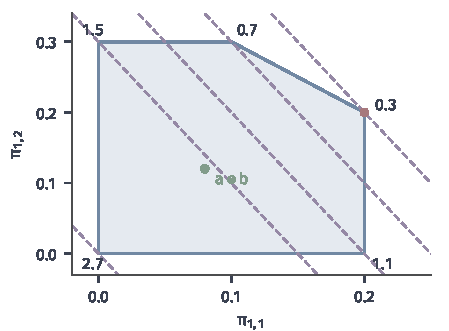
\includegraphics[width=76mm]{figures/07-probability/07-distribution-optimization/matplotlib/ot-polytope/figure.pdf}
 \caption{$\bm{a}=(0.4,0.6)$、$\bm{b}=(0.2,0.3,0.5)$的运输多面体，坐标是$\pi_{1,1}$与$\pi_{1,2}$。浅蓝五边形是可行集，顶点旁的数是该顶点的平方成本；紫色虚线是成本$2.7-8s-4t$的等值线；绿点是独立方案（成本$1.58$），红点是最优顶点（成本$0.3$）。}
 \label{fig:ot-polytope}
\end{BookInlineFigure}

\paragraph{欧氏空间上的分布}
一般分布的耦合集合是无穷维的，需要换一种紧性。第~\ref{chap:weak-convergence-of-distributions}章证明了：$\mathbb{R}^{d}$上一族分布胎紧，则其中任一序列都有弱收敛子列。我们要说明耦合集合正好胎紧，而且弱极限仍是耦合；再说明成本随耦合的变化是下半连续的，即极限处的成本不会突然变大。

\begin{lemma}[耦合集合的紧性]
\label{lem:ot-coupling-compact}
设$\mu,\nu$分别是$\mathbb{R}^{m},\mathbb{R}^{n}$上的概率分布。则$\Pi(\mu,\nu)$胎紧；若$\pi_k\in\Pi(\mu,\nu)$且$\pi_k\xrightarrow{\mathrm{w}}\pi$，则$\pi\in\Pi(\mu,\nu)$。
\end{lemma}

\begin{proof}
任给$\varepsilon>0$。单个分布是胎紧的，取紧集$K_1\subset\mathbb{R}^{m}$与$K_2\subset\mathbb{R}^{n}$，使$\mu(K_1^{\mathrm{c}})<\varepsilon/2$，$\nu(K_2^{\mathrm{c}})<\varepsilon/2$。$K_1\times K_2$是紧集，并且它的补集含于$(K_1^{\mathrm{c}}\times\mathbb{R}^{n})\cup(\mathbb{R}^{m}\times K_2^{\mathrm{c}})$。于是对每个耦合$\pi$，
\[
 \pi\bigl((K_1\times K_2)^{\mathrm{c}}\bigr)\leq\mu(K_1^{\mathrm{c}})+\nu(K_2^{\mathrm{c}})<\varepsilon .
\]
同一个紧集对全部耦合都适用，所以$\Pi(\mu,\nu)$胎紧。

再看弱极限。任取$\mathbb{R}^{m}$上的有界连续函数$h$，函数$(x,y)\mapsto h(x)$在$\mathbb{R}^{m+n}$上有界连续。由弱收敛与第一边缘为$\mu$，
\[
 \int h(x)\,\pi(\mathrm{d}x,\mathrm{d}y)=\lim_{k\to\infty}\int h(x)\,\pi_k(\mathrm{d}x,\mathrm{d}y)=\int h\,\mathrm{d}\mu .
\]
所以$\pi$的第一边缘与$\mu$对一切有界连续函数的积分相同，两者相等。第二边缘同理。
\end{proof}

\begin{lemma}[成本的下半连续性]
\label{lem:ot-cost-lsc}
设$c:\mathbb{R}^{m}\times\mathbb{R}^{n}\to[0,\infty]$是下半连续函数，即对每个点$z$与每个$z_k\to z$有$c(z)\leq\liminf_kc(z_k)$。若概率分布$\pi_k\xrightarrow{\mathrm{w}}\pi$，则
\begin{equation}
 \int c\,\mathrm{d}\pi\leq\liminf_{k\to\infty}\int c\,\mathrm{d}\pi_k .
 \label{eq:ot-cost-lsc}
\end{equation}
\end{lemma}

\begin{proof}
弱收敛只对有界连续函数给出积分的收敛，所以先用有界连续函数从下方逼近$c$。对正整数$j$，令
\[
 c_j(z)=\min\Bigl\{j,\ \inf_{w}\bigl(c(w)+j\lVert z-w\rVert_2\bigr)\Bigr\}.
\]
取$w=z$知$c_j\leq c$；$c_j$关于$j$单调不减，取值在$[0,j]$中。每个$z\mapsto c(w)+j\lVert z-w\rVert_2$都满足$j$-Lipschitz条件，它们的下确界以及与常数$j$的较小者也满足，所以$c_j$连续。

再证$c_j(z)\to c(z)$。任取实数$s<c(z)$。由下半连续，存在$r>0$，使$\lVert w-z\rVert_2<r$时$c(w)>s$。于是对一切$w$，或者$c(w)>s$，或者$j\lVert z-w\rVert_2\geq jr$。当$j\geq\max(s/r,\,s)$时，两种情形下都有
\[
 c(w)+j\lVert z-w\rVert_2\geq s ,
\]
从而$c_j(z)\geq s$。$s$可以任意接近$c(z)$（$c(z)=\infty$时可以任意大），所以$c_j(z)\uparrow c(z)$。

对固定的$j$，$c_j$有界连续，由弱收敛与$c_j\leq c$，
\[
 \int c_j\,\mathrm{d}\pi=\lim_{k\to\infty}\int c_j\,\mathrm{d}\pi_k\leq\liminf_{k\to\infty}\int c\,\mathrm{d}\pi_k .
\]
令$j\to\infty$，由单调收敛定理，左边趋于$\int c\,\mathrm{d}\pi$，得到式~\eqref{eq:ot-cost-lsc}。
\end{proof}

\begin{theorem}[最优耦合的存在]
\label{thm:ot-existence}
设$\mu,\nu$分别是$\mathbb{R}^{m},\mathbb{R}^{n}$上的概率分布，$c:\mathbb{R}^{m}\times\mathbb{R}^{n}\to[0,\infty]$下半连续。则存在$\pi^{*}\in\Pi(\mu,\nu)$，使
\begin{equation}
 \int c\,\mathrm{d}\pi^{*}=\operatorname{OT}_c(\mu,\nu).
 \label{eq:ot-existence}
\end{equation}
\end{theorem}

\begin{proof}
若$\operatorname{OT}_c(\mu,\nu)=\infty$，每个耦合都达到它。下设它有限，取耦合列$\pi_k$，使其成本递减地趋于$\operatorname{OT}_c(\mu,\nu)$。由引理~\ref{lem:ot-coupling-compact}，这列耦合胎紧，由第~\ref{chap:weak-convergence-of-distributions}章的弱收敛子列定理，存在子列$\pi_{k_l}\xrightarrow{\mathrm{w}}\pi^{*}$，并且$\pi^{*}\in\Pi(\mu,\nu)$。由引理~\ref{lem:ot-cost-lsc}，
\[
 \int c\,\mathrm{d}\pi^{*}\leq\liminf_{l\to\infty}\int c\,\mathrm{d}\pi_{k_l}=\operatorname{OT}_c(\mu,\nu).
\]
反向不等式由下确界的定义成立。
\end{proof}

定理的两个条件各有分工。固定边缘使耦合集合胎紧，这是“极小化序列有收敛子列”的来源；下半连续使成本在极限处不会跳高，这是“极限仍是最小者”的来源。$\mathbb{R}^{d}$可以换成一般的完备可分度量空间，证明相同，只是要用一般形式的Prokhorov定理，可查阅~\scite{math-villani2009transport}。

\paragraph{去掉下半连续性}
下面的例子说明下半连续不能省。取$\mu=\nu=\operatorname{Unif}(0,1)$，成本在对角线上取$1$，在对角线外取距离：
\[
 c(x,y)=\begin{cases}1, & x=y,\\ \lvert x-y\rvert, & x\neq y .\end{cases}
\]
它在对角线上不是下半连续的：$c(x,x)=1$，而附近的$c(x,x+h)=\lvert h\rvert\to0$。对$0<h<1$，令$X\sim\operatorname{Unif}(0,1)$，$Y=X+h$（若超过$1$则减去$1$）。$Y$仍服从$\operatorname{Unif}(0,1)$，$X\neq Y$，并且$\lvert X-Y\rvert$以概率$1-h$等于$h$、以概率$h$等于$1-h$，所以成本是
\[
 (1-h)h+h(1-h)=2h(1-h)\to0\qquad(h\to0).
\]
于是$\operatorname{OT}_c(\mu,\nu)=0$。但没有耦合的成本为$0$：若$\pi$在对角线上有正质量，成本至少是这部分质量；若没有，$\pi$的质量全在$\{x\neq y\}$上，$\lvert x-y\rvert>0$处处成立，积分为正。极小化序列弱收敛到对角线上的耦合，成本却在极限处跳到$1$。

\paragraph{耦合存在而映射不达到}
定理只保证最优耦合存在。即使最优耦合存在，Monge问题的下确界也可能取不到。在$\mathbb{R}^{2}$中取$\mu$为线段$\{0\}\times[0,1]$上的均匀分布，$\nu$把一半质量均匀放在$\{-1\}\times[0,1]$上，另一半均匀放在$\{1\}\times[0,1]$上，成本为平方欧氏距离。任何耦合都要把每份质量横向移动距离$1$，所以成本至少为$1$；把每个点的质量平分到左右两侧同一高度，成本恰为$1$，是最优耦合。

映射却做不到$1$。把$[0,1]$等分成$n$段，每段的下半段水平送到左侧、上半段送到右侧，并在竖直方向拉伸两倍铺满该段，得到映射$T_n$。竖直位移在每半段上均匀分布在长为$1/(2n)$的区间里，平均平方为$1/(12n^{2})$，所以$T_n$的成本是
\[
 1+\frac{1}{12n^{2}}\to1 ,
\]
见图~\ref{fig:ot-monge-stripes}。若某个映射$T$的成本恰为$1$，竖直位移必须几乎处处为零，即$T(0,s)=(\pm1,s)$。记$L$为送往左侧的高度集合，左侧收到的质量中高度落在$L$里的部分是$\lvert L\rvert$，而$\nu$要求它是$\lvert L\rvert/2$，所以$\lvert L\rvert=0$；左侧总共却必须收到$1/2$，矛盾。

\begin{BookInlineFigure}
 \centering
 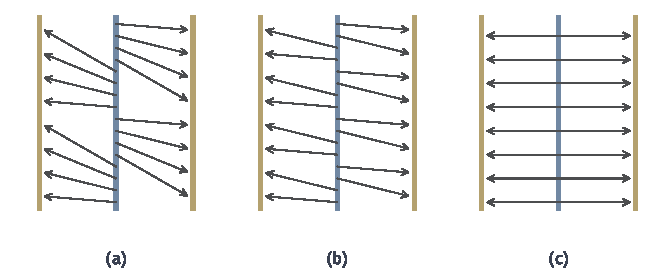
\includegraphics[width=112mm]{figures/07-probability/07-distribution-optimization/matplotlib/ot-monge-stripes/figure.pdf}
 \caption{蓝色竖线是$\mu$（$\{0\}\times[0,1]$上均匀），两条黄色竖线各带$\nu$的一半质量。(a)$n=2$的条带映射$T_2$，成本$1+1/48$。(b)$n=4$的条带映射，成本$1+1/192$。(c)最优耦合把每个点的质量平分到两侧，成本$1$，任何映射都达不到。}
 \label{fig:ot-monge-stripes}
\end{BookInlineFigure}

所以“最优方案存在”只针对耦合。最优耦合能否由映射实现，以及是否唯一，都要另加条件，第~\ref{sec:ot-concrete}节会在具体问题中看到这些条件。

\section{最优性的判别}
\label{sec:ot-optimality}

图~\ref{fig:ot-plan-tables}(c)的逐格搬运成本是$0.6$。怎样确信没有更便宜的方案？逐个比较做不到，可行方案有无穷多个。每个可行方案只给出最优值的一个上界；要证实某个方案最优，还需要一个对一切可行方案都成立的下界，并且它恰好等于这个方案的成本。本节先构造这样的下界，再说明它在什么条件下能与原问题的最优值相等。

\subsection{对偶势}
\label{sec:ot-potentials}

先在有限情形找下界。设想有人提出一组价格：在源位置$x_i$交出一份质量可得收入$f_i$，在目标位置$y_j$收下一份质量可得收入$g_j$。若价格满足
\[
 f_i+g_j\leq c_{i,j}\qquad\text{对一切}\ i,j ,
\]
则无论按什么方案搬运，每份质量带来的收入都不超过它的运费。把行和约束乘以$f_i$、列和约束乘以$g_j$再相加，对任意$\bm{\pi}\in U(\bm{a},\bm{b})$，
\[
 \sum_ia_if_i+\sum_jb_jg_j=\sum_{i,j}\pi_{i,j}(f_i+g_j)\leq\sum_{i,j}\pi_{i,j}c_{i,j} .
\]
左边不依赖方案，所以它是所有可行方案成本的一个公共下界。一般分布的写法相同，只是把向量换成函数。

\begin{definition}[对偶势]
\label{def:ot-potentials}
设$\mu,\nu$与成本$c\geq0$如定义~\ref{def:ot-problem}。若$\varphi\in L^{1}(\mu)$，$\psi\in L^{1}(\nu)$，并且
\begin{equation}
 \varphi(x)+\psi(y)\leq c(x,y)\qquad\text{对一切}\ x\in\mathcal{X},\ y\in\mathcal{Y},
 \label{eq:ot-dual-constraint}
\end{equation}
则称$(\varphi,\psi)$为一对可行的\term{对偶势}（dual potentials），称
\begin{equation}
 J(\varphi,\psi)=\int\varphi\,\mathrm{d}\mu+\int\psi\,\mathrm{d}\nu
 \label{eq:ot-dual-value}
\end{equation}
为它的对偶值。
\end{definition}

对偶势里的$\varphi,\psi$可以取负值，只要求可积；这样它们的积分有限，后面的相减才有意义。下面的定理把“价格”论证写成一般形式，并且给出原对偶值之差的精确表达式。

\begin{theorem}[弱对偶与原对偶差]
\label{thm:ot-weak-duality}
设$(\varphi,\psi)$是可行的对偶势，$\pi\in\Pi(\mu,\nu)$。则
\begin{equation}
 \int c\,\mathrm{d}\pi-J(\varphi,\psi)=\int\bigl(c(x,y)-\varphi(x)-\psi(y)\bigr)\,\pi(\mathrm{d}x,\mathrm{d}y)\geq0 ,
 \label{eq:ot-gap}
\end{equation}
两边可以同时为$+\infty$。于是$J(\varphi,\psi)\leq\operatorname{OT}_c(\mu,\nu)$。若某个$\pi$与$(\varphi,\psi)$使式~\eqref{eq:ot-gap}为零，则$\pi$是最优耦合，$(\varphi,\psi)$使对偶值最大。
\end{theorem}

\begin{proof}
由于$\pi$的第一边缘是$\mu$，对可积的$\varphi$有
\[
 \int\varphi(x)\,\pi(\mathrm{d}x,\mathrm{d}y)=\int\varphi\,\mathrm{d}\mu .
\]
这对示性函数是边缘的定义，对简单函数由线性性成立，对非负函数由单调收敛定理成立，再对正负部分分别使用即得可积情形。$\psi$同理。

记松弛量$s(x,y)=c(x,y)-\varphi(x)-\psi(y)$，由式~\eqref{eq:ot-dual-constraint}它非负，积分有定义。$c=s+\varphi+\psi$中后两项关于$\pi$可积，所以
\[
 \int c\,\mathrm{d}\pi=\int s\,\mathrm{d}\pi+\int\varphi\,\mathrm{d}\mu+\int\psi\,\mathrm{d}\nu ,
\]
这就是式~\eqref{eq:ot-gap}。对$\pi$取下确界得$J(\varphi,\psi)\leq\operatorname{OT}_c(\mu,\nu)$。若差为零，$\pi$的成本等于一个下界，不可能有成本更低的耦合；对任何别的可行对偶势$(\varphi',\psi')$，由刚证明的不等式，$J(\varphi',\psi')$不超过$\int c\,\mathrm{d}\pi$，而后者等于$J(\varphi,\psi)$。
\end{proof}

式~\eqref{eq:ot-gap}的右边只看$\pi$把质量放在哪里：放在松弛量为零的地方不贡献差，放在松弛量为正的地方按松弛量计差。所以候选方案$\pi$的最优性可以这样核验：找一对可行的对偶势，检查$\pi$的质量是否几乎全部落在等号集合$\{c=\varphi+\psi\}$上。这一条件称为互补松弛。

\paragraph{例子的证据}
回到全章例子。取
\[
 \bm{f}=(0,\ -1,\ -2),\qquad \bm{g}=(0,\ 1,\ 2),
\]
则$f_i+g_j=j-i$。成本$(i-j)^{2}$与它的差就是松弛矩阵
\[
 \bm{S}=\bm{C}-\bigl(f_i+g_j\bigr)_{i,j}=\begin{bmatrix}0&0&2\\2&0&0\\6&2&0\end{bmatrix}.
\]
各元素非负，所以$(\bm{f},\bm{g})$可行；对偶值为
\[
 \langle\bm{a},\bm{f}\rangle+\langle\bm{b},\bm{g}\rangle=(-0.3-0.4)+(0.3+1.0)=0.6 .
\]
逐格搬运的质量放在$(0,0),(0,1),(1,2),(2,2)$上，这四处的松弛量都是$0$，于是它的成本$0.6$等于这个下界，它是最优方案。

同一对势也给出其他方案离最优有多远。由式~\eqref{eq:ot-gap}，跳格搬运把$0.3$放在松弛量为$2$的$(0,2)$处，所以
\[
 1.2-0.6=0.3\times2 .
\]
独立方案在每个格子上都有质量，它与最优值之差是$\sum_{i,j}a_ib_js_{i,j}$，逐项相加得
\[
 0.25\times2+0.06\times2+0.04\times6+0.06\times2=0.98=1.58-0.6 .
\]
图~\ref{fig:ot-dual-envelope}(b)画出松弛矩阵，红圈标出最优方案的质量所在。

\paragraph{由一个势求另一个势}
给定$\bm{g}$，满足约束的$f_i$最大能取多少？约束$f_i\leq c_{i,j}-g_j$对每个$j$成立，所以最大可取
\begin{equation}
 f_i=\min_{j}\bigl(c_{i,j}-g_j\bigr).
 \label{eq:ot-c-transform}
\end{equation}
这称为$\bm{g}$的\term{$c$变换}（$c$-transform）；一般情形写成$\psi^{c}(x)=\inf_y\bigl(c(x,y)-\psi(y)\bigr)$。对偶值关于$\bm{f}$单调增加，所以最优的$\bm{f}$总可以取成$\bm{g}$的$c$变换。几何上，它是一族曲线$x\mapsto c(x,y_j)-g_j$的下包络。图~\ref{fig:ot-dual-envelope}(a)对例子中的$\bm{g}=(0,1,2)$画出三条抛物线$(x-j)^{2}-j$与它们的下包络，在$x=0,1,2$处恰好取到$\bm{f}=(0,-1,-2)$。

\begin{BookInlineFigure}
 \centering
 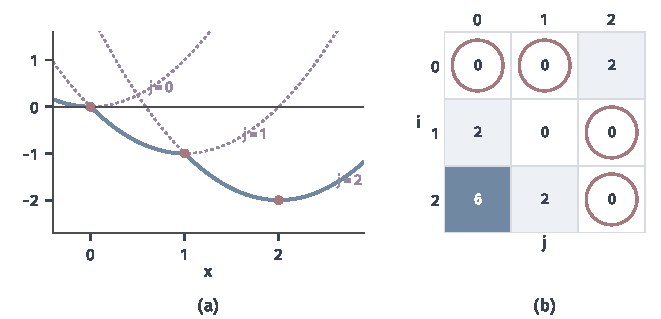
\includegraphics[width=112mm]{figures/07-probability/07-distribution-optimization/matplotlib/ot-dual-envelope/figure.pdf}
 \caption{全章例子的对偶势。(a)紫色点线是$(x-j)^{2}-g_j$，$\bm{g}=(0,1,2)$；蓝线是它们的下包络，即$\bm{g}$的$c$变换；红点是$f_i$。(b)松弛量$c_{i,j}-f_i-g_j$，红圈是逐格搬运方案的非零位置，全部落在零松弛处。}
 \label{fig:ot-dual-envelope}
\end{BookInlineFigure}

成本取度量$d$时，$c$变换产生第~\ref{chap:distribution-comparison}章的Lipschitz函数：$\psi^{c}(x)=\inf_y(d(x,y)-\psi(y))$是一族$1$-Lipschitz函数的下确界，本身也是$1$-Lipschitz函数。再对一个$1$-Lipschitz函数$h$求$c$变换，由$h(y)-h(x)\leq d(x,y)$得$\inf_y(d(x,y)-h(y))\geq-h(x)$，取$y=x$取等，结果恰为$-h$。所以对偶势可以取成$(-h,h)$的形式，对偶值是$\mathbb{E}_{\nu}[h]-\mathbb{E}_{\mu}[h]$；Kantorovich--Rubinstein对偶正是一般对偶在$c=d$时的这一特殊形式。

最优势一般不唯一。例子中把$\bm{f}$加上常数$t$、$\bm{g}$减去$t$，对偶值不变；即使固定$f_0=0$，可行最优势也不止一组。由零松弛的四个位置得$g_0=0$，$g_1=1$，$g_2=1-f_1$，$f_2=f_1-1$，再检查其余五个约束，得到$-3\leq f_1\leq-1$，其中每个$f_1$都给出对偶值$0.6$。最优方案唯一（第~\ref{sec:ot-one-dimensional}节将证明），证明它最优的价格却有许多组。

\subsection{强对偶的条件}
\label{sec:ot-strong-duality}

弱对偶只给出不等式。要用对偶势证实最优性，还需要知道下界能够逼近甚至等于最优值，即两个问题之间没有\term{对偶间隙}（duality gap）。先证明有限情形。

\begin{theorem}[有限运输问题的强对偶]
\label{thm:ot-finite-duality}
设$\bm{a}\in\mathbb{R}^{m}$，$\bm{b}\in\mathbb{R}^{n}$是概率向量，$\bm{C}\in\mathbb{R}^{m\times n}$。则
\begin{equation}
 \min_{\bm{\pi}\in U(\bm{a},\bm{b})}\langle\bm{C},\bm{\pi}\rangle=\max\Bigl\{\langle\bm{a},\bm{f}\rangle+\langle\bm{b},\bm{g}\rangle:\ f_i+g_j\leq c_{i,j}\ \text{对一切}\ i,j\Bigr\},
 \label{eq:ot-finite-duality}
\end{equation}
两边的最小值与最大值都能取到。
\end{theorem}

\begin{proof}
把$\bm{\pi}$的$mn$个元素看成变量。原问题是线性规划：在等式约束$\sum_j\pi_{i,j}=a_i$（$m$个）、$\sum_i\pi_{i,j}=b_j$（$n$个）和$\pi_{i,j}\geq0$下最小化$\sum_{i,j}c_{i,j}\pi_{i,j}$。给前$m$个等式配乘子$f_i$，后$n$个配乘子$g_j$，Lagrange函数是
\[
 \sum_{i,j}c_{i,j}\pi_{i,j}+\sum_if_i\Bigl(a_i-\sum_j\pi_{i,j}\Bigr)+\sum_jg_j\Bigl(b_j-\sum_i\pi_{i,j}\Bigr).
\]
整理成
\[
 \langle\bm{a},\bm{f}\rangle+\langle\bm{b},\bm{g}\rangle+\sum_{i,j}\bigl(c_{i,j}-f_i-g_j\bigr)\pi_{i,j} .
\]
对$\pi_{i,j}\geq0$取下确界，只有当每个系数$c_{i,j}-f_i-g_j$都非负时下确界才有限，等于$\langle\bm{a},\bm{f}\rangle+\langle\bm{b},\bm{g}\rangle$。所以对偶线性规划正是式~\eqref{eq:ot-finite-duality}右边。

原问题可行（含$\bm{a}\bm{b}^{\top}$），目标值不小于$\min_{i,j}c_{i,j}$，有下界。由线性规划的强对偶定理，原问题与对偶问题都有最优解，并且最优值相等，可参考\BookChapterRef{chap:linear-programming}{卷五第2章“线性规划”}。
\end{proof}

第~\ref{chap:distribution-comparison}章证明有限支撑的Kantorovich--Rubinstein对偶，用的正是这个定理。一般分布不能直接套用线性规划，但在紧致空间上可以用有限问题去逼近。

\begin{theorem}[紧致空间上的强对偶]
\label{thm:ot-compact-duality}
设$(\mathcal{X},d_{\mathcal{X}})$，$(\mathcal{Y},d_{\mathcal{Y}})$是紧致度量空间，$c:\mathcal{X}\times\mathcal{Y}\to[0,\infty)$连续，$\mu,\nu$分别是其上的Borel概率分布。则
\begin{equation}
 \operatorname{OT}_c(\mu,\nu)=\sup\bigl\{J(\varphi,\psi):\ (\varphi,\psi)\ \text{是有界可测的可行对偶势}\bigr\}.
 \label{eq:ot-compact-duality}
\end{equation}
\end{theorem}

\begin{proof}
由定理~\ref{thm:ot-weak-duality}，右边不超过左边，只需对每个$\eta>0$构造对偶值不小于$\operatorname{OT}_c(\mu,\nu)-3\eta$的可行势。

\emph{第一步：选尺度。}$\mathcal{X}\times\mathcal{Y}$紧致，$c$在其上一致连续：存在$\delta>0$，使$d_{\mathcal{X}}(x,x')<\delta$且$d_{\mathcal{Y}}(y,y')<\delta$时$\lvert c(x,y)-c(x',y')\rvert\leq\eta$。

\emph{第二步：离散化。}紧致空间可被有限个半径$\delta/2$的球覆盖，依次去掉与前面重叠的部分并丢弃空集，得到$\mathcal{X}$的有限Borel划分$A_1,\dots,A_m$，每块直径小于$\delta$；同样得到$\mathcal{Y}$的划分$B_1,\dots,B_n$。在每块中取一个代表点$x_i\in A_i$，$y_j\in B_j$，令
\[
 a_i=\mu(A_i),\qquad b_j=\nu(B_j),\qquad c_{i,j}=c(x_i,y_j).
\]
由定理~\ref{thm:ot-finite-duality}，离散问题有最优方案$\bm{\pi}^{\delta}$与最优对偶解$(\bm{f},\bm{g})$，两者的值相等，记为$V_\delta$。

\emph{第三步：离散问题不比原问题贵太多。}把离散方案铺回原空间：在$A_i\times B_j$上放入质量$\pi^{\delta}_{i,j}$，并按$\mu$与$\nu$在这两块上的形状分布，即
\[
 \pi=\sum_{i,j:\ a_i>0,\ b_j>0}\pi^{\delta}_{i,j}\,\frac{\mu|_{A_i}}{a_i}\otimes\frac{\nu|_{B_j}}{b_j} .
\]
（$a_i=0$时第$i$行全为零，可以略去。）由行和$\sum_j\pi^{\delta}_{i,j}=a_i$，它的第一边缘是
\[
 \sum_i\Bigl(\sum_j\pi^{\delta}_{i,j}\Bigr)\frac{\mu|_{A_i}}{a_i}=\sum_i\mu|_{A_i}=\mu ,
\]
第二边缘同理是$\nu$，所以$\pi\in\Pi(\mu,\nu)$。在$A_i\times B_j$上$c\leq c_{i,j}+\eta$，于是
\[
 \operatorname{OT}_c(\mu,\nu)\leq\int c\,\mathrm{d}\pi\leq V_\delta+\eta .
\]

\emph{第四步：把离散势扩展成函数。}令
\[
 \varphi(x)=\min_{j}\bigl(c(x,y_j)-g_j\bigr),\qquad \psi(y)=g_j-\eta\quad(y\in B_j).
\]
$\varphi$是有限个连续函数的最小值，$\psi$是简单函数，都有界可测。可行性：对$y\in B_j$，$\lvert c(x,y_j)-c(x,y)\rvert\leq\eta$，所以
\[
 \varphi(x)+\psi(y)\leq c(x,y_j)-g_j+g_j-\eta\leq c(x,y).
\]
对偶值：对$x\in A_i$，$c(x,y_j)\geq c_{i,j}-\eta$，又由离散对偶可行性$c_{i,j}-g_j\geq f_i$，所以$\varphi(x)\geq f_i-\eta$。于是
\[
 J(\varphi,\psi)\geq\sum_ia_i(f_i-\eta)+\sum_jb_j(g_j-\eta)=V_\delta-2\eta .
\]
与第三步合起来，
\[
 J(\varphi,\psi)\geq\operatorname{OT}_c(\mu,\nu)-3\eta .
\]
\end{proof}

证明的每一步都在利用紧致性。一致连续使“在同一小块里换一个点”只改变成本$\eta$；有限覆盖使离散问题是有限线性规划；连续成本有界，使势函数有界。证明得到的是“无对偶间隙”：对偶值可以任意接近原问题的最优值。它没有说上确界被某对势函数取到。在这些条件下最优势其实存在，可以取成一对互为$c$变换的连续函数，证明要从一列近似势中用Arzelà--Ascoli定理抽出一致收敛子列，可查阅~\scite{math-villani2009transport}。

\paragraph{离开紧致与连续}
三个结论需要分别核对。原问题的最小值被取到，靠的是第~\ref{sec:ot-existence}节的胎紧与成本下半连续；无对偶间隙，在完备可分度量空间上对非负下半连续成本仍成立，此时可以只用有界连续的对偶势；最优势的存在，还要求成本被可积函数控制，例如存在$\alpha\in L^{1}(\mu)$与$\beta\in L^{1}(\nu)$使$c(x,y)\leq\alpha(x)+\beta(y)$，平方成本与有限二阶矩就是这种情形。这些一般结论的证明可查阅前面提到的Villani的专著。

三者不能互相代替。第~\ref{sec:ot-existence}节的非下半连续例子中，$\varphi=\psi=0$是可行势，对偶值$0$等于最优值，没有对偶间隙，可是原问题取不到最小值。所以，用对偶势证实一个具体方案最优，需要的不仅是“没有间隙”，而是手中的方案与势恰好使式~\eqref{eq:ot-gap}为零。

\section{具体运输问题}
\label{sec:ot-concrete}

前两节回答了最优耦合何时存在、怎样证实。真正把它求出来，要靠问题本身的结构。本节看三类结构：实数轴上的顺序使最优方案“不交叉”，可以由分位数直接写出；有限支持使问题成为线性规划；高斯分布与平方成本的二次结构使最优方案是一个仿射映射。每个问题都要回答两件事：最优成本是多少，以及最优方案是一般耦合还是由映射产生。

\subsection{一维分布}
\label{sec:ot-one-dimensional}

在实数轴上，交叉的搬运总是浪费。设$x_1<x_2$两处各有一份质量，要送到$y_1<y_2$。交叉配对把$x_1$送到$y_2$、$x_2$送到$y_1$，顺序配对则$x_1\to y_1$、$x_2\to y_2$，见图~\ref{fig:ot-uncross}。对凸的成本$h(x-y)$，顺序配对不会更贵：交叉配对的两个位移$x_1-y_2$与$x_2-y_1$一个最小、一个最大，顺序配对的两个位移夹在中间且总和相同，凸函数在两端的和不小于在中间的和。这启发我们：最优方案应当按顺序配对，把源分布的第$u$分位数送到目标分布的第$u$分位数。

\begin{BookInlineFigure}
 \centering
 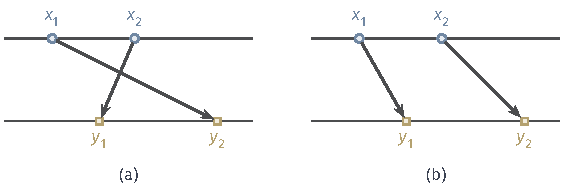
\includegraphics[width=96mm]{figures/07-probability/07-distribution-optimization/tikz/ot-uncross/figure.pdf}
 \caption{实数轴上的交换论证。上方是源点$x_1<x_2$（蓝），下方是目标点$y_1<y_2$（黄）。(a)交叉配对。(b)顺序配对。对凸成本$h(x-y)$，(b)的成本不超过(a)。}
 \label{fig:ot-uncross}
\end{BookInlineFigure}

\paragraph{分位数耦合}
设$\mu,\nu$是实数轴上的分布，分布函数为$F,G$。沿用第~\ref{chap:random-variables}章的广义分位数$F^{-1}(u)=\inf\{x:F(x)\geq u\}$，$0<u<1$，它满足
\[
 F^{-1}(u)\leq x\quad\Longleftrightarrow\quad u\leq F(x).
\]
取$U\sim\operatorname{Unif}(0,1)$，令$X=F^{-1}(U)$，$Y=G^{-1}(U)$。由上面的等价关系，$\mathbb{P}(X\leq x)=\mathbb{P}(U\leq F(x))=F(x)$，所以$X\sim\mu$；同理$Y\sim\nu$。$(X,Y)$的联合分布因此是$\mu$与$\nu$的一个耦合，称为\term{分位数耦合}（quantile coupling）。它的联合分布函数是
\begin{equation}
 \mathbb{P}(X\leq s,\ Y\leq t)=\mathbb{P}\bigl(U\leq F(s),\ U\leq G(t)\bigr)=\min\bigl(F(s),G(t)\bigr).
 \label{eq:ot-comonotone-cdf}
\end{equation}
两个分量由同一个$U$单调地决定，$U$越大两者都越大，所以这个耦合“不交叉”。

\begin{theorem}[一维最优运输]
\label{thm:ot-one-dimensional}
设$\mu,\nu$是实数轴上具有有限$p$阶矩的分布，$p\geq1$，分布函数为$F,G$，成本$c(x,y)=\lvert x-y\rvert^{p}$。则分位数耦合是最优耦合，
\begin{equation}
 W_p^{p}(\mu,\nu)=\int_0^{1}\bigl\lvert F^{-1}(u)-G^{-1}(u)\bigr\rvert^{p}\,\mathrm{d}u .
 \label{eq:ot-quantile-formula}
\end{equation}
$p=1$时还有
\begin{equation}
 W_1(\mu,\nu)=\int_{-\infty}^{\infty}\bigl\lvert F(x)-G(x)\bigr\rvert\,\mathrm{d}x .
 \label{eq:ot-cdf-formula}
\end{equation}
$p>1$时最优耦合唯一。
\end{theorem}

$p=1$与$p>1$的证明思路不同。$p=1$时成本对距离是线性的，可以把$\lvert x-y\rvert$拆成对阈值的积分，直接得到下界；$p>1$时先由第~\ref{sec:ot-existence}节取得一个最优耦合，再证明它必定不交叉，不交叉的耦合只有分位数耦合一个。

\begin{proof}[$p=1$的证明]
对实数$x,y$，示性函数$\mathbf{1}_{\{x\leq t\}}$与$\mathbf{1}_{\{y\leq t\}}$只在$t$介于$x,y$之间时不同，所以
\[
 \lvert x-y\rvert=\int_{-\infty}^{\infty}\bigl\lvert\mathbf{1}_{\{x\leq t\}}-\mathbf{1}_{\{y\leq t\}}\bigr\rvert\,\mathrm{d}t .
\]
任取耦合$(X,Y)$，两边取期望，被积函数非负，由Tonelli定理交换期望与积分，再对每个$t$用“绝对值的期望不小于期望的绝对值”，
\[
 \mathbb{E}\lvert X-Y\rvert=\int_{-\infty}^{\infty}\mathbb{E}\bigl\lvert\mathbf{1}_{\{X\leq t\}}-\mathbf{1}_{\{Y\leq t\}}\bigr\rvert\,\mathrm{d}t\geq\int_{-\infty}^{\infty}\lvert F(t)-G(t)\rvert\,\mathrm{d}t .
\]
所以式~\eqref{eq:ot-cdf-formula}右边是一切耦合成本的下界。

对分位数耦合，$\{X\leq t\}=\{U\leq F(t)\}$，$\{Y\leq t\}=\{U\leq G(t)\}$，两个事件一个包含另一个，所以
\[
 \mathbb{E}\bigl\lvert\mathbf{1}_{\{X\leq t\}}-\mathbf{1}_{\{Y\leq t\}}\bigr\rvert=\bigl\lvert F(t)-G(t)\bigr\rvert ,
\]
上面的不等式取等。分位数耦合达到下界，是最优耦合，并且$W_1$同时等于式~\eqref{eq:ot-quantile-formula}与式~\eqref{eq:ot-cdf-formula}的右边。
\end{proof}

式~\eqref{eq:ot-cdf-formula}说的是：$W_1$等于两条分布函数曲线之间的面积。式~\eqref{eq:ot-quantile-formula}说的是同一块面积换一个方向切片：按纵坐标$u$切成水平条，每条的长度是$\lvert F^{-1}(u)-G^{-1}(u)\rvert$。图~\ref{fig:ot-quantile-coupling}对全章例子画出两种看法。

$p>1$的证明需要一个关于最优耦合支撑的引理。$\mathbb{R}^{2}$上分布$\pi$的支撑是这样的点$z$的全体：以$z$为中心的每个开球都有正的$\pi$质量。支撑之外的点各有一个零质量邻域，这些邻域可以由可数个有理中心、有理半径的零质量球覆盖，所以支撑之外的总质量为零；换句话说，正质量的集合一定与支撑相交。

\begin{lemma}[最优耦合不能局部改进]
\label{lem:ot-two-point}
设$c:\mathbb{R}\times\mathbb{R}\to[0,\infty)$连续，$\pi$是$\mu,\nu$的成本有限的最优耦合。则对$\pi$支撑中的任意两点$(x_1,y_1),(x_2,y_2)$，
\begin{equation}
 c(x_1,y_1)+c(x_2,y_2)\leq c(x_1,y_2)+c(x_2,y_1).
 \label{eq:ot-two-point}
\end{equation}
\end{lemma}

\begin{proof}
设两点不同而不等式反向，差为$3\eta>0$。由连续性，可取$\delta>0$，使两个开方块
\[
 Q_k=(x_k-\delta,x_k+\delta)\times(y_k-\delta,y_k+\delta),\qquad k=1,2
\]
互不相交，并且只要$(x,y)\in Q_1$，$(x',y')\in Q_2$，就有
\[
 c(x,y)+c(x',y')\geq c(x,y')+c(x',y)+\eta .
\]
两点在支撑中，$m_k=\pi(Q_k)>0$。记$\pi_k=\pi|_{Q_k}/m_k$，它的两个边缘为$\alpha_k,\beta_k$。取$\lambda=\min(m_1,m_2)$，构造
\[
 \pi'=\pi-\lambda(\pi_1+\pi_2)+\lambda\bigl(\alpha_1\otimes\beta_2+\alpha_2\otimes\beta_1\bigr).
\]
在$Q_k$上$\pi\geq m_k\pi_k\geq\lambda\pi_k$，所以$\pi'$非负。第一边缘先减去$\lambda(\alpha_1+\alpha_2)$、再加回$\lambda(\alpha_1+\alpha_2)$，没有改变，第二边缘同理，于是$\pi'\in\Pi(\mu,\nu)$。这一步把两块中的质量“交换目的地”：$Q_1$里的源送往$Q_2$里的目标，反之亦然。成本的改变量是
\[
 \begin{aligned}
 &\lambda\iint\bigl(c(x,y')+c(x',y)-c(x,y)-c(x',y')\bigr)\,\pi_1(\mathrm{d}x,\mathrm{d}y)\,\pi_2(\mathrm{d}x',\mathrm{d}y')\\
 &\qquad\leq-\lambda\eta<0 ,
 \end{aligned}
\]
其中各项积分有限，因为$c$在有界集上有界。这与$\pi$最优矛盾。
\end{proof}

\begin{proof}[$p>1$的证明]
有限$p$阶矩保证独立耦合的成本有限，成本连续，由定理~\ref{thm:ot-existence}，最优耦合存在。任取一个最优耦合$\pi$，我们证明它就是分位数耦合，于是分位数耦合最优，而且最优耦合唯一。

\emph{第一步：支撑不交叉。}设支撑中有$(x_1,y_1),(x_2,y_2)$满足$x_1<x_2$而$y_1>y_2$。记
\[
 r=x_1-y_1,\qquad v=x_1-y_2,\qquad w=x_2-y_1,\qquad z=x_2-y_2 .
\]
则$v,w$都严格介于$r$与$z$之间，并且
\[
 v+w=r+z .
\]
令$\lambda=(z-v)/(z-r)\in(0,1)$，则
\[
 v=\lambda r+(1-\lambda)z,\qquad w=(1-\lambda)r+\lambda z .
\]
$h(s)=\lvert s\rvert^{p}$在$p>1$时严格凸，所以
\[
 h(v)+h(w)<\lambda h(r)+(1-\lambda)h(z)+(1-\lambda)h(r)+\lambda h(z)=h(r)+h(z),
\]
即$c(x_1,y_2)+c(x_2,y_1)<c(x_1,y_1)+c(x_2,y_2)$，与引理~\ref{lem:ot-two-point}矛盾。所以支撑中$x_1<x_2$蕴含$y_1\leq y_2$。

\emph{第二步：不交叉决定联合分布。}任取$s,t$。若事件$\{x\leq s,\,y>t\}$与$\{x>s,\,y\leq t\}$的$\pi$质量都为正，两者都与支撑相交，得到支撑中的点$(x_1,y_1)$、$(x_2,y_2)$，满足$x_1\leq s<x_2$且$y_2\leq t<y_1$，与第一步矛盾。所以两者至少有一个质量为零。若前者为零，
\[
 \pi(x\leq s,\,y\leq t)=\pi(x\leq s)=F(s),
\]
又因为它不超过$\pi(y\leq t)=G(t)$，它等于$\min(F(s),G(t))$。后者为零时同理。于是$\pi$的联合分布函数就是式~\eqref{eq:ot-comonotone-cdf}，二维分布由联合分布函数唯一确定，$\pi$等于分位数耦合。
\end{proof}

$p=1$时最优耦合一般不唯一。第~\ref{chap:distribution-comparison}章已经看到，例表上逐格搬运与跳格搬运的一阶成本相同；这正是$h(s)=\lvert s\rvert$不严格凸的结果，交换论证中的不等式可以取等。

\paragraph{例子的计算}
全章例子的两个分布函数与分位数函数分别是阶梯函数。$F$在$0,1,2$处跳到$0.5,0.8,1$，$G$跳到$0.2,0.5,1$。把$(0,1)$按两组跳跃高度切开，得到四个区间：
\[
 (0,0.2],\qquad(0.2,0.5],\qquad(0.5,0.8],\qquad(0.8,1).
\]
在这四段上$(F^{-1}(u),G^{-1}(u))$依次取$(0,0)$、$(0,1)$、$(1,2)$、$(2,2)$，各段长度$0.2,0.3,0.3,0.2$就是分位数耦合放在这些点对上的质量，它正是图~\ref{fig:ot-plan-tables}(c)的逐格搬运。由定理~\ref{thm:ot-one-dimensional}，逐格搬运是平方成本下唯一的最优方案，这印证了上一节用对偶势得到的结论。由式~\eqref{eq:ot-cdf-formula}，
\[
 W_1=\int_0^{1}(0.5-0.2)\,\mathrm{d}x+\int_1^{2}(0.8-0.5)\,\mathrm{d}x=0.6 ,
\]
这证明了第~\ref{chap:distribution-comparison}章提到的关系：$W_1$等于两条分布函数之间的面积。由式~\eqref{eq:ot-quantile-formula}，
\[
 W_2^{2}=0.3\times1^{2}+0.3\times1^{2}=0.6 .
\]

\begin{BookInlineFigure}
 \centering
 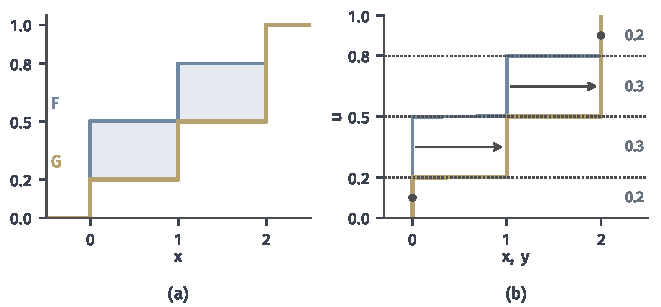
\includegraphics[width=112mm]{figures/07-probability/07-distribution-optimization/matplotlib/ot-quantile-coupling/figure.pdf}
 \caption{全章例子的一维运输。(a)$F$（蓝）与$G$（黄），两者之间浅蓝区域的面积是$W_1=0.6$。(b)分位数函数，横轴为取值，纵轴为$u$；虚线把$(0,1)$分成四段，每段内箭头从$F^{-1}(u)$指向$G^{-1}(u)$，右侧数字是该段长度，即搬运的质量；黑点表示质量留在原地。}
 \label{fig:ot-quantile-coupling}
\end{BookInlineFigure}

\paragraph{何时由映射实现}
分位数耦合是$U$的函数对，但不一定是$X$的函数。若$F$连续，它是。先说明$F(X)\sim\operatorname{Unif}(0,1)$：由分位数的等价关系，$F(x)\geq u$当且仅当$x\geq F^{-1}(u)$，而$F$连续时$\mathbb{P}(X=F^{-1}(u))=0$且$F(F^{-1}(u))=u$，所以
\[
 \mathbb{P}\bigl(F(X)\geq u\bigr)=\mathbb{P}\bigl(X\geq F^{-1}(u)\bigr)=1-u .
\]
再说明$F^{-1}(F(X))=X$几乎必然成立：总有$F^{-1}(F(x))\leq x$，严格小于只发生在$F$的平台上，平台的质量为零。于是取$U=F(X)$，分位数耦合就是$(X,\,G^{-1}(F(X)))$，
\begin{equation}
 T=G^{-1}\circ F
 \label{eq:ot-monotone-map}
\end{equation}
是一个单调不减的最优运输映射。

源分布有原子时，分位数耦合必须把原子拆开。取
\[
 \mu=\tfrac12\delta_0+\tfrac12\operatorname{Unif}(1,2),\qquad \nu=\operatorname{Unif}(0,2),
\]
则
\[
 F^{-1}(u)=\begin{cases}0, & u\leq\tfrac12,\\ 2u, & u>\tfrac12,\end{cases}\qquad G^{-1}(u)=2u .
\]
$u\leq\tfrac12$时，$0$处的原子被均匀地铺到$[0,1]$上；$u>\tfrac12$时质量不动。由式~\eqref{eq:ot-quantile-formula}，
\[
 W_1=\int_0^{1/2}2u\,\mathrm{d}u=\frac14,\qquad W_2^{2}=\int_0^{1/2}4u^{2}\,\mathrm{d}u=\frac16 .
\]
$W_1$也等于图~\ref{fig:ot-atom-quantile}(a)中$F$与$G$之间三角形的面积$\tfrac12\times1\times\tfrac12$。这里不存在任何运输映射：映射把$0$处质量为$\tfrac12$的原子整体送到一个点，像分布就有质量至少$\tfrac12$的原子，而$\nu$没有原子。分位数配对总能定义耦合，却未必给出源点的单值映射。

\begin{BookInlineFigure}
 \centering
 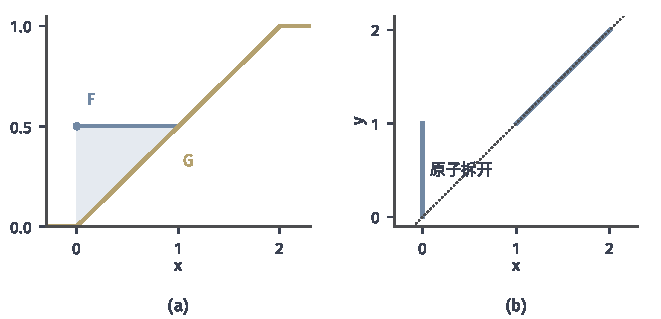
\includegraphics[width=112mm]{figures/07-probability/07-distribution-optimization/matplotlib/ot-atom-quantile/figure.pdf}
 \caption{带原子的源分布$\mu=\tfrac12\delta_0+\tfrac12\operatorname{Unif}(1,2)$与$\nu=\operatorname{Unif}(0,2)$。(a)$F$（蓝）与$G$（黄），在$[1,2]$上两者重合；浅蓝三角形面积$W_1=1/4$。(b)分位数耦合的支撑：$x=0$处的竖线表示原子被铺到$[0,1]$上，$[1,2]$上的斜线表示质量不动。}
 \label{fig:ot-atom-quantile}
\end{BookInlineFigure}

\subsection{离散运输}
\label{sec:ot-discrete}

高维的有限问题没有顺序可用，只能直接解线性规划。把$\bm{\pi}$排成长为$mn$的向量，问题是$m+n$个等式约束、$mn$个非负变量的线性规划。行约束之和与列约束之和都等于总质量$1$，所以等式约束中有一个是多余的，独立的约束是$m+n-1$个。

\paragraph{顶点的结构}
由前面提到的线性规划理论，线性规划若有最优解，就有一个最优解是可行集合的顶点。运输多面体的顶点有简单的组合刻画。把$\bm{\pi}$的非零位置看成二部图的边：左边是源点，右边是目标点，$\pi_{i,j}>0$时连接$i$与$j$。若这些边含有一个圈$i_1\to j_1\to i_2\to j_2\to\cdots\to i_1$，沿圈交替地对各边加上和减去一个小量$\epsilon$，每个点上一加一减，行和列和不变。于是$\bm{\pi}$是两个可行方案$\bm{\pi}\pm\epsilon\bm{D}$的中点，不是顶点。所以顶点的非零位置不含圈，构成一个森林，边数至多是点数减一，即
\[
 \#\{(i,j):\pi_{i,j}>0\}\leq m+n-1 .
\]
最优顶点因此很稀疏，但稀疏不等于一一配对：$m\neq n$时一一配对根本不可能，$m=n$时一个源点也可能把质量分给几个目标点。

当$m=n$且$\bm{a}=\bm{b}=\tfrac1n\bm{1}$时，顶点恰好是置换矩阵除以$n$。森林中总有只连一条边的点，比如第$i$行只有一个非零元$\pi_{i,j}$，它必须等于行和$\tfrac1n$，于是第$j$列也已满额；删去这一行一列，剩下的仍是同类问题，归纳下去即得。这时最优运输就是\term{指派问题}（assignment problem），可参考\BookChapterRef{chap:bipartite-matching-assignment}{卷三第6章“二部图匹配与指派”}。

\paragraph{网络流的视角}
运输问题也是一个最小费用流问题：从每个源点$i$流出$a_i$，流入每个目标点$j$恰好$b_j$，弧$(i,j)$上单位流量的费用是$c_{i,j}$，没有容量上限。网络单纯形法在可行生成树之间移动，正是在运输多面体的顶点之间移动；它维护的节点势就是本章的对偶势，判断最优的“没有负费用圈”等价于所有松弛量非负。这些方法可参考\BookChapterRef{chap:min-cost-flow}{卷三第7章“最小费用流”}。

\paragraph{平面上的例子}
取平面上的三个源点与四个目标点，成本为平方欧氏距离：
\[
 \begin{aligned}
 &x_1=(0,0),\quad x_2=(0,2),\quad x_3=(3,1),\\
 &\bm{a}=(0.4,\ 0.4,\ 0.2),\\
 &y_1=(1,0),\quad y_2=(2,2),\quad y_3=(4,0),\quad y_4=(1,3),\\
 &\bm{b}=(0.3,\ 0.3,\ 0.2,\ 0.2).
 \end{aligned}
\]
成本矩阵与一个最优方案是
\[
 \bm{C}=\begin{bmatrix}1&8&16&10\\5&4&20&2\\5&2&2&8\end{bmatrix},\qquad
 \bm{\pi}^{*}=\begin{bmatrix}0.3&0.1&0&0\\0&0.2&0&0.2\\0&0&0.2&0\end{bmatrix},
\]
成本是
\[
 0.3\times1+0.1\times8+0.2\times4+0.2\times2+0.2\times2=2.7 .
\]
图~\ref{fig:ot-lp-plane}画出这个方案。$x_1$的质量分给了$y_1$与$y_2$，$y_2$从两个源点收货；非零元有$5$个，少于$m+n-1=6$，是一个退化的顶点。

\begin{BookInlineFigure}
 \centering
 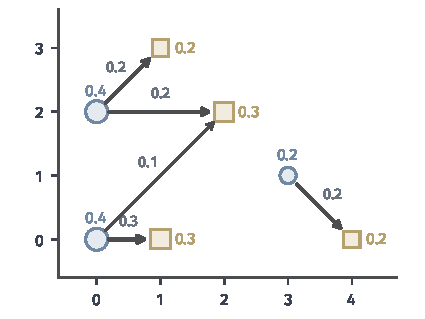
\includegraphics[width=72mm]{figures/07-probability/07-distribution-optimization/matplotlib/ot-lp-plane/figure.pdf}
 \caption{平面上的离散运输，平方欧氏成本。蓝圆是源点，黄方块是目标点，旁边的数是质量；箭头是最优方案的非零元，粗细与箭头旁的数表示搬运的质量。最优成本为$2.7$。}
 \label{fig:ot-lp-plane}
\end{BookInlineFigure}

\paragraph{结果的检验}
线性规划求解器输出的方案要逐项检验，不能只看目标值。检验三件事。第一，非负性：$\min_{i,j}\pi_{i,j}\geq0$。第二，边缘残差：行和与$\bm{a}$之差、列和与$\bm{b}$之差的$\ell_1$范数之和应为零，数值解应在容差以内；不满足边缘约束的方案，其成本不是最优值的上界。第三，原对偶差：再给出一对势$(\bm{f},\bm{g})$，检查对偶可行性$\max_{i,j}(f_i+g_j-c_{i,j})\leq0$，并计算$\langle\bm{C},\bm{\pi}\rangle-\langle\bm{a},\bm{f}\rangle-\langle\bm{b},\bm{g}\rangle$。由式~\eqref{eq:ot-gap}，前两项满足时这个差非负并且控制方案与最优值的距离。

对上面的例子，令$f_1=0$，在非零位置上解$f_i+g_j=c_{i,j}$，得$g_1=1$，$g_2=8$，$f_2=-4$，$g_4=6$；第三个源点只连$y_3$，自成一棵树，$f_3+g_3=2$还有一个自由度，取$f_3=-6$，$g_3=8$。于是
\[
 \bm{f}=(0,\ -4,\ -6),\qquad \bm{g}=(1,\ 8,\ 8,\ 6),
\]
松弛矩阵是
\[
 \bm{C}-\bigl(f_i+g_j\bigr)_{i,j}=\begin{bmatrix}0&0&8&4\\8&0&16&0\\10&0&0&8\end{bmatrix}\geq0 ,
\]
对偶值是
\[
 \langle\bm{a},\bm{f}\rangle+\langle\bm{b},\bm{g}\rangle=-2.8+5.5=2.7 ,
\]
原对偶差为零，$\bm{\pi}^{*}$最优。它也是唯一的最优方案：零松弛位置只有$(1,1),(1,2),(2,2),(2,4),(3,2),(3,3)$，第三列只有$(3,3)$一处零松弛，所以第三个源点的$0.2$必须全部给$y_3$，$(3,2)$只能为零；其余位置随之唯一确定。

\subsection{高斯分布的二次运输}
\label{sec:ot-gaussian}

在$\mathbb{R}^{d}$上取平方欧氏成本，$c(x,y)=\lVert x-y\rVert_2^{2}$。先把均值分离出去。设$X\sim\mu$，$Y\sim\nu$，均值分别是$\bm{m}_1,\bm{m}_2$，二阶矩有限，记$\tilde{X}=X-\bm{m}_1$，$\tilde{Y}=Y-\bm{m}_2$。对任意耦合，
\[
 \mathbb{E}\lVert X-Y\rVert_2^{2}=\lVert\bm{m}_1-\bm{m}_2\rVert_2^{2}+2\bigl\langle\bm{m}_1-\bm{m}_2,\ \mathbb{E}[\tilde{X}-\tilde{Y}]\bigr\rangle+\mathbb{E}\lVert\tilde{X}-\tilde{Y}\rVert_2^{2},
\]
中间项为零。所以平方运输成本等于均值之差的平方加上把两个中心化分布对齐的成本，两部分互不影响。中心化部分再展开，
\[
 \mathbb{E}\lVert\tilde{X}-\tilde{Y}\rVert_2^{2}=\operatorname{tr}\bm{\Sigma}_1+\operatorname{tr}\bm{\Sigma}_2-2\,\mathbb{E}\langle\tilde{X},\tilde{Y}\rangle ,
\]
其中$\bm{\Sigma}_1,\bm{\Sigma}_2$是协方差矩阵。前两项只依赖边缘，所以最小化成本就是最大化$\mathbb{E}\langle\tilde{X},\tilde{Y}\rangle$：让两个向量尽可能“同向”。

\begin{theorem}[高斯分布的平方运输]
\label{thm:ot-gaussian}
设$\mu=\mathcal{N}(\bm{m}_1,\bm{\Sigma}_1)$，$\nu=\mathcal{N}(\bm{m}_2,\bm{\Sigma}_2)$，两个协方差矩阵都正定。令
\begin{equation}
 \bm{A}=\bm{\Sigma}_1^{-1/2}\bigl(\bm{\Sigma}_1^{1/2}\bm{\Sigma}_2\bm{\Sigma}_1^{1/2}\bigr)^{1/2}\bm{\Sigma}_1^{-1/2},\qquad T(x)=\bm{m}_2+\bm{A}(x-\bm{m}_1).
 \label{eq:ot-gaussian-map}
\end{equation}
则$T$是从$\mu$到$\nu$的最优运输映射，并且
\begin{equation}
 W_2^{2}(\mu,\nu)=\lVert\bm{m}_1-\bm{m}_2\rVert_2^{2}+\operatorname{tr}\bm{\Sigma}_1+\operatorname{tr}\bm{\Sigma}_2-2\operatorname{tr}\bigl(\bm{\Sigma}_1^{1/2}\bm{\Sigma}_2\bm{\Sigma}_1^{1/2}\bigr)^{1/2}.
 \label{eq:ot-gaussian-w2}
\end{equation}
\end{theorem}

这里的平方根都是对称正定矩阵的唯一对称正定平方根。记$\bm{M}$为式~\eqref{eq:ot-gaussian-map}中括号的平方根，它对称正定；$\bm{A}$是对称正定矩阵与它的合同变换，仍对称正定。

\begin{proof}
\emph{映射可行。}$T$是仿射映射，$T(X)$是高斯向量，均值为$\bm{m}_2$，协方差为
\[
 \bm{A}\bm{\Sigma}_1\bm{A}=\bm{\Sigma}_1^{-1/2}\bm{M}\bm{\Sigma}_1^{-1/2}\bm{\Sigma}_1\bm{\Sigma}_1^{-1/2}\bm{M}\bm{\Sigma}_1^{-1/2}=\bm{\Sigma}_1^{-1/2}\bm{M}^{2}\bm{\Sigma}_1^{-1/2}=\bm{\Sigma}_2 .
\]
所以$T_\#\mu=\nu$。

\emph{映射最优。}由前面的分解，只需证明对中心化的任意耦合$(\tilde{X},\tilde{Y})$，内积的期望$\mathbb{E}\langle\tilde{X},\tilde{Y}\rangle$不超过$\tilde{Y}=\bm{A}\tilde{X}$时的值。对任意向量$x,y$，
\[
 \tfrac12\langle x,\bm{A}x\rangle+\tfrac12\langle y,\bm{A}^{-1}y\rangle-\langle x,y\rangle=\tfrac12\bigl\lVert\bm{A}^{1/2}x-\bm{A}^{-1/2}y\bigr\rVert_2^{2}\geq0 ,
\]
等号当且仅当$y=\bm{A}x$。代入$x=\tilde{X}$，$y=\tilde{Y}$并取期望，
\[
 \mathbb{E}\langle\tilde{X},\tilde{Y}\rangle\leq\tfrac12\operatorname{tr}(\bm{A}\bm{\Sigma}_1)+\tfrac12\operatorname{tr}(\bm{A}^{-1}\bm{\Sigma}_2).
\]
右边只依赖两个边缘，是一切耦合的公共上界；$\tilde{Y}=\bm{A}\tilde{X}$时取等，而这正是$T$给出的耦合。

\emph{成本。}在$T$给出的耦合下，$\mathbb{E}\langle\tilde{X},\bm{A}\tilde{X}\rangle$等于$\operatorname{tr}(\bm{A}\bm{\Sigma}_1)$，并且
\[
 \operatorname{tr}(\bm{A}\bm{\Sigma}_1)=\operatorname{tr}\bigl(\bm{\Sigma}_1^{-1/2}\bm{M}\bm{\Sigma}_1^{1/2}\bigr)=\operatorname{tr}\bm{M} .
\]
代入前面的分解即得式~\eqref{eq:ot-gaussian-w2}。
\end{proof}

证明中的二次型不等式是凸函数$\tfrac12\langle x,\bm{A}x\rangle$与它的凸共轭之间的Fenchel--Young不等式。一般地，平方成本下的最优映射是某个凸函数的梯度，这里的凸函数是二次函数，梯度就是对称正定的线性映射$\bm{A}$。对称性是关键：同样把$\mu$推成$\nu$的映射还有许多，但只有对称正定的那一个是最优的。

一维时式~\eqref{eq:ot-gaussian-w2}化为
\begin{equation}
 W_2^{2}\bigl(\mathcal{N}(m_1,\sigma_1^{2}),\mathcal{N}(m_2,\sigma_2^{2})\bigr)=(m_1-m_2)^{2}+(\sigma_1-\sigma_2)^{2},
 \label{eq:ot-gaussian-1d}
\end{equation}
最优映射是$T(x)=m_2+(\sigma_2/\sigma_1)(x-m_1)$，也就是第~\ref{sec:ot-one-dimensional}节的$G^{-1}\circ F$。

\paragraph{一个能手算的例子}
取$\mu=\mathcal{N}(\bm{0},\bm{I})$，$\nu=\mathcal{N}(\bm{m},\bm{\Sigma}_2)$，其中
\[
 \bm{m}=(3,\ 1),\qquad \bm{\Sigma}_2=\operatorname{diag}\bigl(4,\ \tfrac14\bigr).
\]
$\bm{\Sigma}_1=\bm{I}$，所以$\bm{A}=\bm{M}=\bm{\Sigma}_2^{1/2}$，即$\operatorname{diag}(2,\tfrac12)$，最优映射是
\[
 T(x)=(3,\ 1)+\bigl(2x_1,\ \tfrac12x_2\bigr).
\]
由式~\eqref{eq:ot-gaussian-w2}，
\[
 W_2^{2}=10+2+\tfrac{17}{4}-2\bigl(2+\tfrac12\bigr)=10+1.25=11.25 ,
\]
均值移动贡献$10$，形状改变贡献$(1-2)^{2}+(1-\tfrac12)^{2}=1.25$。

作为对照，先把$x$旋转$90^{\circ}$再拉伸：
\[
 T'(x)=\bm{m}+\operatorname{diag}\bigl(2,\tfrac12\bigr)\bm{R}x,\qquad \bm{R}=\begin{bmatrix}0&-1\\1&0\end{bmatrix}.
\]$\bm{R}\bm{R}^{\top}=\bm{I}$，所以$T'(X)$的协方差仍是$\bm{\Sigma}_2$，$T'$也是运输映射。它的成本是
\[
 10+\operatorname{tr}\bm{I}+\operatorname{tr}\bm{\Sigma}_2-2\operatorname{tr}\bigl(\operatorname{diag}(2,\tfrac12)\bm{R}\bigr)=10+2+4.25-0=16.25 .
\]
$\operatorname{diag}(2,\tfrac12)\bm{R}$不对称，对角线为零，它让$\tilde{X}$与$\tilde{Y}$完全不同向。图~\ref{fig:ot-gaussian-map}对比了两个映射：红点$(1,0)$在最优映射下送到$(5,1)$，在$T'$下送到$(3,\tfrac32)$。

\begin{BookInlineFigure}
 \centering
 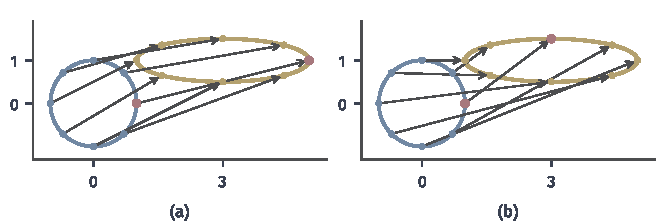
\includegraphics[width=112mm]{figures/07-probability/07-distribution-optimization/matplotlib/ot-gaussian-map/figure.pdf}
 \caption{$\mathcal{N}(\bm{0},\bm{I})$（蓝圈为单位标准差等高线）到$\mathcal{N}((3,1),\operatorname{diag}(4,\tfrac14))$（黄椭圆）。箭头是圆上八个点的像，红点是$(1,0)$及其像。(a)最优映射$T(x)=\bm{m}+\operatorname{diag}(2,\tfrac12)x$，成本$11.25$。(b)先旋转$90^{\circ}$再拉伸的映射，像分布相同，成本$16.25$。}
 \label{fig:ot-gaussian-map}
\end{BookInlineFigure}

\paragraph{奇异协方差}
定理要求$\bm{\Sigma}_1$可逆，因为$\bm{A}$的公式含$\bm{\Sigma}_1^{-1/2}$。源分布退化时，最优耦合与最优成本仍可研究，但必须按支撑子空间检查映射是否可行。取$d=2$，
\[
 \mu=\mathcal{N}\bigl(\bm{0},\operatorname{diag}(1,0)\bigr),\qquad \nu=\mathcal{N}(\bm{0},\bm{I}).
\]
$\mu$集中在横轴上，$X=(X_1,0)$。两者均值都是零，由前面的分解，最小化成本就是最大化$\mathbb{E}\langle X,Y\rangle$。对任意耦合，由Cauchy--Schwarz不等式，
\[
 \mathbb{E}\langle X,Y\rangle=\mathbb{E}[X_1Y_1]\leq\sqrt{\mathbb{E}X_1^{2}\,\mathbb{E}Y_1^{2}}=1 ,
\]
等号当且仅当$Y_1=X_1$。于是最优耦合必须让$Y_1=X_1$，而$Y_2$要服从$\mathcal{N}(0,1)$并且与$Y_1$独立（$\nu$的两个分量独立），所以最优耦合唯一：
\[
 Y=(X_1,\ Z),\qquad Z\sim\mathcal{N}(0,1)\ \text{与}\ X_1\ \text{独立},
\]
成本是$\mathbb{E}Z^{2}=1$。$Y_2$与$X$独立，不是$X$的函数，所以最优耦合不由映射产生，见图~\ref{fig:ot-gaussian-singular}。

反方向的问题落在定理~\ref{thm:ot-gaussian}之内。把两个分布对调，以$\nu$为源，它的协方差可逆，式~\eqref{eq:ot-gaussian-w2}给出
\[
 0+2+1-2\operatorname{tr}\operatorname{diag}(1,0)=1 ,
\]
与直接计算一致；对调方向的最优映射是投影$(y_1,y_2)\mapsto(y_1,0)$。协方差奇异时式~\eqref{eq:ot-gaussian-w2}本身仍然成立，可以用正定情形取极限得到，但不能把含$\bm{\Sigma}_1^{-1/2}$的映射公式直接套用。

\begin{BookInlineFigure}
 \centering
 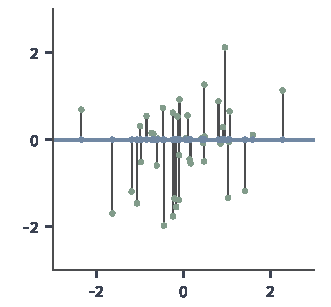
\includegraphics[width=56mm]{figures/07-probability/07-distribution-optimization/matplotlib/ot-gaussian-singular/figure.pdf}
 \caption{退化源分布$\mathcal{N}(\bm{0},\operatorname{diag}(1,0))$（蓝线为其支撑）到$\mathcal{N}(\bm{0},\bm{I})$的唯一最优耦合，$40$对模拟点，种子$729$。蓝点是源点，绿点是目标点，竖线是搬运路径：每份质量只沿竖直方向移动，目标高度与源点独立。}
 \label{fig:ot-gaussian-singular}
\end{BookInlineFigure}

\section{熵正则化}
\label{sec:ot-entropic}

$m$个源点、$n$个目标点的运输线性规划有$mn$个变量。分布由细网格离散化时，$m,n$成千上万，单纯形类方法要在巨大的多面体顶点之间移动，而且最优解落在边界上，对数据的微小变化不连续。一个常用的办法是在成本上加一个惩罚，鼓励方案“散开”一些：散开的方案位于多面体内部，最优性条件变成光滑的方程，可以用简单的交替缩放求解。代价是求得的不再是原问题的最优方案。本节研究这一权衡。

\paragraph{正则化问题}
设$\bm{a}\in\mathbb{R}^{m}$，$\bm{b}\in\mathbb{R}^{n}$是概率向量。若某个$a_i=0$，任何可行方案的第$i$行都必须为零，这一行可以直接删去；对$b_j=0$的列也一样。所以下面总设$\bm{a},\bm{b}$的各分量都为正。以边缘乘积$\bm{a}\otimes\bm{b}$，即独立方案$(a_ib_j)_{i,j}$为参考，对$\varepsilon>0$考虑
\begin{equation}
 \min_{\bm{\pi}\in U(\bm{a},\bm{b})}\ L_\varepsilon(\bm{\pi}),\qquad L_\varepsilon(\bm{\pi})=\langle\bm{C},\bm{\pi}\rangle+\varepsilon D_{\mathrm{KL}}(\bm{\pi}\Vert\bm{a}\otimes\bm{b}),
 \label{eq:ot-entropic-problem}
\end{equation}
其中
\[
 D_{\mathrm{KL}}(\bm{\pi}\Vert\bm{a}\otimes\bm{b})=\sum_{i,j}\pi_{i,j}\ln\frac{\pi_{i,j}}{a_ib_j},
\]
约定$0\ln0=0$。这一问题称为\term{熵正则化最优运输}（entropic optimal transport）。

两项各有含义。$\langle\bm{C},\bm{\pi}\rangle$是原来的运输成本；KL项是方案偏离独立方案的程度。把$\bm{\pi}$看成$(X,Y)$的联合分布，它的两个边缘是$\bm{a},\bm{b}$，所以这一项正是第~\ref{chap:information-measures}章的互信息$I(X;Y)$：它衡量知道源位置后，对目标位置的不确定性减少了多少。$\varepsilon$很大时，惩罚迫使方案接近独立方案，源与目标几乎无关；$\varepsilon\to0$时，方案回到原问题的最优方案，源几乎决定目标。图~\ref{fig:ot-entropic-plans}在一个细网格上展示这一变化。

\begin{BookInlineFigure}
 \centering
 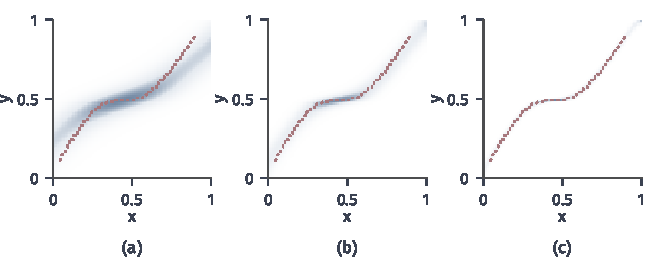
\includegraphics[width=112mm]{figures/07-probability/07-distribution-optimization/matplotlib/ot-entropic-plans/figure.pdf}
 \caption{$[0,1]$上$80$个格点的熵正则化方案，源为双峰分布，目标为单峰分布，平方成本。图中是按行归一化后的方案，即给定$x$时$y$的条件分布，颜色越深概率越大；红色点线是不加正则化时的单调最优映射。(a)$\varepsilon=0.02$。(b)$\varepsilon=0.005$。(c)$\varepsilon=0.0005$。}
 \label{fig:ot-entropic-plans}
\end{BookInlineFigure}

\paragraph{对偶问题与原对偶差}
正则化问题的对偶变量仍是一对向量$\bm{f}\in\mathbb{R}^{m}$，$\bm{g}\in\mathbb{R}^{n}$，但约束$f_i+g_j\leq c_{i,j}$换成一个光滑的惩罚：
\begin{equation}
 D_\varepsilon(\bm{f},\bm{g})=\langle\bm{a},\bm{f}\rangle+\langle\bm{b},\bm{g}\rangle-\varepsilon\sum_{i,j}a_ib_j\Bigl(\mathrm{e}^{(f_i+g_j-c_{i,j})/\varepsilon}-1\Bigr).
 \label{eq:ot-entropic-dual}
\end{equation}
违反约束越多，指数项越大；$\varepsilon\to0$时，它趋于“满足约束为$0$、违反约束为$-\infty$”的硬约束。下面的引理是第~\ref{sec:ot-potentials}节式~\eqref{eq:ot-gap}的对应物。

\begin{lemma}[正则化问题的原对偶差]
\label{lem:ot-entropic-gap}
对$\bm{\pi}\in U(\bm{a},\bm{b})$与任意$\bm{f},\bm{g}$，记$r_{i,j}=\pi_{i,j}/(a_ib_j)$，$s_{i,j}=(f_i+g_j-c_{i,j})/\varepsilon$。则
\begin{equation}
 L_\varepsilon(\bm{\pi})-D_\varepsilon(\bm{f},\bm{g})=\varepsilon\sum_{i,j}a_ib_j\bigl(r_{i,j}\ln r_{i,j}-r_{i,j}-r_{i,j}s_{i,j}+\mathrm{e}^{s_{i,j}}\bigr)\geq0 ,
 \label{eq:ot-entropic-gap}
\end{equation}
每一项取等当且仅当$r_{i,j}=\mathrm{e}^{s_{i,j}}$。
\end{lemma}

\begin{proof}
由行列约束，
\[
 \langle\bm{a},\bm{f}\rangle+\langle\bm{b},\bm{g}\rangle=\sum_{i,j}\pi_{i,j}(f_i+g_j);
\]
又$\bm{a}\otimes\bm{b}$与$\bm{\pi}$的元素总和都是$1$。代入式~\eqref{eq:ot-entropic-dual}，
\[
 L_\varepsilon(\bm{\pi})-D_\varepsilon(\bm{f},\bm{g})=\sum_{i,j}\pi_{i,j}(c_{i,j}-f_i-g_j)+\varepsilon\sum_{i,j}\pi_{i,j}\ln r_{i,j}+\varepsilon\sum_{i,j}a_ib_j\mathrm{e}^{s_{i,j}}-\varepsilon .
\]
把$\pi_{i,j}(c_{i,j}-f_i-g_j)$写成$-\varepsilon a_ib_jr_{i,j}s_{i,j}$，把常数$\varepsilon$写成$\varepsilon\sum_{i,j}a_ib_jr_{i,j}$，即得等式。

对固定的$r\geq0$，函数$s\mapsto\mathrm{e}^{s}-rs$在$r>0$时于$s=\ln r$处取最小值$r-r\ln r$，所以
\[
 r\ln r-r-rs+\mathrm{e}^{s}\geq r\ln r-r+r-r\ln r=0 ,
\]
等号当且仅当$s=\ln r$；$r=0$时这一项是$\mathrm{e}^{s}>0$。
\end{proof}

\begin{theorem}[熵正则化问题的解]
\label{thm:ot-entropic-solution}
设$\bm{a},\bm{b}$各分量为正，$\bm{C}$各元素有限，$\varepsilon>0$。则问题~\eqref{eq:ot-entropic-problem}有唯一解$\bm{\pi}^{\varepsilon}$，它的各元素都为正，并且存在$\bm{f},\bm{g}$使
\begin{equation}
 \pi^{\varepsilon}_{i,j}=a_ib_j\,\mathrm{e}^{(f_i+g_j-c_{i,j})/\varepsilon}.
 \label{eq:ot-entropic-form}
\end{equation}
这样的$(\bm{f},\bm{g})$使$D_\varepsilon$取最大值，并且最大值等于$L_\varepsilon(\bm{\pi}^{\varepsilon})$。反过来，$U(\bm{a},\bm{b})$中任何形如式~\eqref{eq:ot-entropic-form}的方案都是唯一解。
\end{theorem}

\begin{proof}
\emph{存在与唯一。}$t\mapsto t\ln t$在$[0,\infty)$上连续，所以$L_\varepsilon$在紧集$U(\bm{a},\bm{b})$上连续，最小值取得。$t\mapsto t\ln(t/(a_ib_j))$严格凸，成本项是线性的，所以$L_\varepsilon$在凸集$U(\bm{a},\bm{b})$上严格凸，最小点唯一。

\emph{各元素为正。}设可行的$\bm{\pi}$有零元素。对$0<\lambda<1$令
\[
 \bm{\pi}^{\lambda}=(1-\lambda)\bm{\pi}+\lambda\,\bm{a}\otimes\bm{b},
\]
它是两个可行方案的凸组合，仍可行。成本项与$\bm{\pi}$的正元素对应的熵项都是$\lambda$的可微函数，它们的变化不超过$K\lambda$（$K$为常数，$\lambda$足够小）。$\bm{\pi}$的零元素$(i,j)$处，熵项从$0$变为
\[
 \lambda a_ib_j\ln\frac{\lambda a_ib_j}{a_ib_j}=\lambda a_ib_j\ln\lambda .
\]
记$\kappa>0$为零元素处$a_ib_j$之和，则
\[
 L_\varepsilon(\bm{\pi}^{\lambda})-L_\varepsilon(\bm{\pi})\leq\lambda\bigl(K+\varepsilon\kappa\ln\lambda\bigr),
\]
$\lambda$足够小时右边为负。所以有零元素的方案不是最小点。

\emph{缩放形式。}最小点$\bm{\pi}^{\varepsilon}$各元素为正，对任何行和、列和都为零的矩阵$\bm{D}$，$\bm{\pi}^{\varepsilon}+t\bm{D}$在$\lvert t\rvert$很小时可行。$t\mapsto L_\varepsilon(\bm{\pi}^{\varepsilon}+t\bm{D})$在$t=0$处取最小，导数为零：
\[
 \sum_{i,j}D_{i,j}h_{i,j}=0,\qquad h_{i,j}=c_{i,j}+\varepsilon\ln\frac{\pi^{\varepsilon}_{i,j}}{a_ib_j}+\varepsilon .
\]
对$i<m$，$j<n$取$\bm{D}$在$(i,j),(m,n)$处为$1$、在$(i,n),(m,j)$处为$-1$、其余为$0$，它的行和、列和都是零，代入得
\[
 h_{i,j}=(h_{i,n}-h_{m,n})+h_{m,j} .
\]
令$\alpha_i=h_{i,n}-h_{m,n}$，$\beta_j=h_{m,j}$，可以逐一核对$h_{i,j}=\alpha_i+\beta_j$对包括末行末列在内的一切$i,j$成立。取$f_i=\alpha_i-\varepsilon$，$g_j=\beta_j$，解出$\pi^{\varepsilon}_{i,j}$即得式~\eqref{eq:ot-entropic-form}。

\emph{对偶。}式~\eqref{eq:ot-entropic-form}说的就是$r_{i,j}=\mathrm{e}^{s_{i,j}}$，由引理~\ref{lem:ot-entropic-gap}，原对偶差为零。对任何$(\bm{f}',\bm{g}')$，同一引理说明它的对偶值不超过$L_\varepsilon(\bm{\pi}^{\varepsilon})$，而$(\bm{f},\bm{g})$的对偶值等于它，所以$(\bm{f},\bm{g})$使$D_\varepsilon$最大。反过来，可行且形如式~\eqref{eq:ot-entropic-form}的方案使原对偶差为零，它的$L_\varepsilon$值等于一个下界，是最小点。
\end{proof}

记$u_i=\mathrm{e}^{f_i/\varepsilon}$，$v_j=\mathrm{e}^{g_j/\varepsilon}$，以及正矩阵
\begin{equation}
 K_{i,j}=a_ib_j\,\mathrm{e}^{-c_{i,j}/\varepsilon},
 \label{eq:ot-gibbs-kernel}
\end{equation}
式~\eqref{eq:ot-entropic-form}写成
\begin{equation}
 \bm{\pi}^{\varepsilon}=\operatorname{diag}(\bm{u})\,\bm{K}\operatorname{diag}(\bm{v}).
 \label{eq:ot-scaling-form}
\end{equation}正则化解是固定矩阵$\bm{K}$的行与列分别乘上一个正因子。问题于是变成：找正向量$\bm{u},\bm{v}$，使缩放后的矩阵行和为$\bm{a}$、列和为$\bm{b}$。

\paragraph{正则化目标与运输成本}
正则化问题的解给出两个数：正则化目标值$L_\varepsilon(\bm{\pi}^{\varepsilon})$，以及它的运输成本$\langle\bm{C},\bm{\pi}^{\varepsilon}\rangle$。两者都不等于原问题的最优值$\operatorname{OT}$，必须分开记录。设$\bm{\pi}^{*}$是原问题的一个最优方案。$\bm{\pi}^{\varepsilon}$使$L_\varepsilon$最小，所以它的$L_\varepsilon$值不超过$\bm{\pi}^{*}$的值；再利用KL非负，
\begin{equation}
 0\leq\langle\bm{C},\bm{\pi}^{\varepsilon}\rangle-\operatorname{OT}\leq\varepsilon D_{\mathrm{KL}}(\bm{\pi}^{*}\Vert\bm{a}\otimes\bm{b})\leq\varepsilon\min\bigl(H(\bm{a}),H(\bm{b})\bigr),
 \label{eq:ot-entropic-bias}
\end{equation}
熵以奈特计。左边的不等式是因为$\bm{\pi}^{\varepsilon}$可行；最后一步是因为互信息不超过任一边缘的熵（第~\ref{chap:information-measures}章）。所以运输成本的偏差随$\varepsilon$线性地趋于零。

全章例子中，$\bm{\pi}^{*}$是逐格搬运，
\[
 \begin{aligned}
 D_{\mathrm{KL}}(\bm{\pi}^{*}\Vert\bm{a}\otimes\bm{b})&=2\times0.2\ln\frac{0.2}{0.1}+2\times0.3\ln\frac{0.3}{0.15}\\
 &=\ln2\approx0.693 .
 \end{aligned}
\]
$\varepsilon=1$时数值求得$\langle\bm{C},\bm{\pi}^{\varepsilon}\rangle\approx0.814$，偏差$0.214$，在上界$0.693$之内；正则化目标值约为$1.087$，比运输成本还多出$\varepsilon D_{\mathrm{KL}}(\bm{\pi}^{\varepsilon}\Vert\bm{a}\otimes\bm{b})\approx0.272$。图~\ref{fig:ot-entropic-bias}画出两者随$\varepsilon$的变化：$\varepsilon\to\infty$时运输成本趋于独立方案的$1.58$，$\varepsilon\to0$时趋于$0.6$。

\begin{BookInlineFigure}
 \centering
 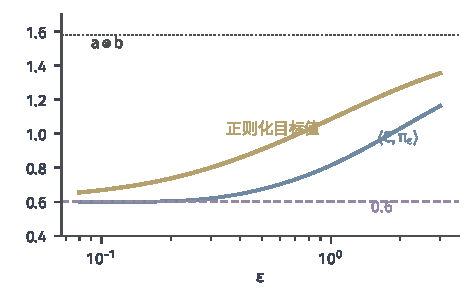
\includegraphics[width=80mm]{figures/07-probability/07-distribution-optimization/matplotlib/ot-entropic-bias/figure.pdf}
 \caption{全章例子的熵正则化偏差，横轴为$\varepsilon$（对数刻度）。蓝线是正则化解的运输成本$\langle\bm{C},\bm{\pi}^{\varepsilon}\rangle$，黄线是正则化目标值$L_\varepsilon(\bm{\pi}^{\varepsilon})$，紫色虚线是原问题最优值$0.6$，深灰点线是独立方案的成本$1.58$。}
 \label{fig:ot-entropic-bias}
\end{BookInlineFigure}

\subsection{Sinkhorn迭代}
\label{sec:ot-sinkhorn}

要找的是两个缩放向量。若列因子$\bm{v}$已知，行条件$\sum_ju_iK_{i,j}v_j=a_i$对每个$i$只含一个未知数$u_i$，立即解出；反过来，行因子已知时列因子也立即解出。于是交替地做这两件事。

\paragraph{交替缩放}
固定$\bm{v}$，令行和等于$\bm{a}$；再固定新的$\bm{u}$，令列和等于$\bm{b}$：
\begin{equation}
 u_i\leftarrow\frac{a_i}{(\bm{K}\bm{v})_i},\qquad v_j\leftarrow\frac{b_j}{(\bm{K}^{\top}\bm{u})_j}.
 \label{eq:ot-sinkhorn}
\end{equation}
这一迭代称为\term{Sinkhorn迭代}（Sinkhorn iteration）。每半步只满足一组约束，并破坏另一组；交替进行时，两组约束的残差逐步减小。

每半步还有一个优化含义。对式~\eqref{eq:ot-entropic-dual}关于$f_i$求偏导，
\[
 \frac{\partial D_\varepsilon}{\partial f_i}=a_i-\sum_ja_ib_j\mathrm{e}^{(f_i+g_j-c_{i,j})/\varepsilon}=a_i-\sum_ju_iK_{i,j}v_j .
\]
令它为零，就是式~\eqref{eq:ot-sinkhorn}的行更新。$D_\varepsilon$关于$\bm{f}$是凹函数，所以行更新在$\bm{g}$固定时把$D_\varepsilon$对$\bm{f}$精确地最大化，列更新同理。Sinkhorn迭代是对偶问题的交替坐标上升，对偶值逐步增大。

\paragraph{对数域计算}
$\varepsilon$很小时$\mathrm{e}^{-c_{i,j}/\varepsilon}$会下溢为零，$u_i,v_j$则会上溢。改用$\bm{f}=\varepsilon\ln\bm{u}$，$\bm{g}=\varepsilon\ln\bm{v}$表示，行更新中的$a_i$与$K_{i,j}$里的$a_i$相消，得到
\begin{equation}
 f_i\leftarrow-\varepsilon\ln\sum_jb_j\,\mathrm{e}^{(g_j-c_{i,j})/\varepsilon},\qquad g_j\leftarrow-\varepsilon\ln\sum_ia_i\,\mathrm{e}^{(f_i-c_{i,j})/\varepsilon}.
 \label{eq:ot-sinkhorn-log}
\end{equation}
计算$\ln\sum_j\exp(z_j)$时先减去$\max_jz_j$再求指数，结果再加回，所有指数都不超过$1$，不会溢出。式~\eqref{eq:ot-sinkhorn-log}是$c$变换~\eqref{eq:ot-c-transform}的光滑版本：$\varepsilon\to0$时，$-\varepsilon\ln\sum_jb_j\mathrm{e}^{(g_j-c_{i,j})/\varepsilon}$趋于$\min_j(c_{i,j}-g_j)$。

\paragraph{停止判据}
每轮做完列更新后，列和精确等于$\bm{b}$，行和与$\bm{a}$的差$\rho=\lVert\bm{\pi}\bm{1}-\bm{a}\rVert_1$衡量可行性。但当前方案不可行，它的目标值不能直接与最优值比较。为此先把它修成一个可行方案$\tilde{\bm{\pi}}$：行和超过$a_i$的行按比例缩小到$a_i$；列和超过$b_j$的列同样缩小；此时行缺额$\bm{e}_r=\bm{a}-\tilde{\bm{\pi}}\bm{1}$与列缺额$\bm{e}_c=\bm{b}-\tilde{\bm{\pi}}^{\top}\bm{1}$都非负且总和相等，再加上$\bm{e}_r\bm{e}_c^{\top}/\lVert\bm{e}_r\rVert_1$补足。由引理~\ref{lem:ot-entropic-gap}与定理~\ref{thm:ot-entropic-solution}，
\begin{equation}
 0\leq L_\varepsilon(\tilde{\bm{\pi}})-L_\varepsilon(\bm{\pi}^{\varepsilon})\leq L_\varepsilon(\tilde{\bm{\pi}})-D_\varepsilon(\bm{f},\bm{g}),
 \label{eq:ot-sinkhorn-stop}
\end{equation}
右边可以直接算出。它小于容差$\tau$时停止，输出$\tilde{\bm{\pi}}$，并且知道它与正则化最优值的差不超过$\tau$。

\needspace{6\baselineskip}
\paragraph{变量}
\begin{itemize}
 \item $\bm{K}\in\mathbb{R}^{m\times n}$：式~\eqref{eq:ot-gibbs-kernel}的正矩阵，计算一次后不变。
 \item $\bm{u}\in\mathbb{R}^{m}$，$\bm{v}\in\mathbb{R}^{n}$：行、列缩放因子，在原处更新；对数域中改存$\bm{f},\bm{g}$。
 \item $\bm{\pi}^{(t)}\in\mathbb{R}^{m\times n}$：第$t$轮列更新后按式~\eqref{eq:ot-scaling-form}组成的方案，列和为$\bm{b}$。
 \item $\rho^{(t)}$：行残差；$\tilde{\bm{\pi}}^{(t)}$：修正后的可行方案；$\Delta^{(t)}$：式~\eqref{eq:ot-sinkhorn-stop}右边的原对偶差。
 \item $\tau$：容差；$T_{\max}$：最大轮数。
\end{itemize}

\paragraph{初始化}
令$\bm{v}=\bm{1}$（即$\bm{g}=\bm{0}$），轮次$t=0$。下面用全章例子演示，取$\varepsilon=1$，$\tau=10^{-4}$。由式~\eqref{eq:ot-gibbs-kernel}，
\[
 \bm{K}=\begin{bmatrix}0.1000&0.0552&0.0046\\0.0221&0.0900&0.0552\\0.0007&0.0221&0.1000\end{bmatrix},
\]
例如$K_{0,1}=0.5\times0.3\times\mathrm{e}^{-1}$。表中数值保留四位小数，计算按全精度进行。

\needspace{6\baselineskip}
\paragraph{每轮更新}
第$t$轮：
\begin{enumerate}
 \item \textbf{行缩放。}按式~\eqref{eq:ot-sinkhorn}计算$u_i=a_i/(\bm{K}\bm{v})_i$。例中第一轮$\bm{v}=\bm{1}$，$\bm{K}\bm{v}$是$\bm{K}$的行和，
 \[
  \bm{K}\bm{v}=(0.1598,\ 0.1673,\ 0.1228),\qquad \bm{u}=(3.1297,\ 1.7937,\ 1.6286).
 \]

 \item \textbf{列缩放。}按式~\eqref{eq:ot-sinkhorn}计算$v_j=b_j/(\bm{K}^{\top}\bm{u})_j$。例中第一轮
 \[
  \bm{K}^{\top}\bm{u}=(0.3538,\ 0.3701,\ 0.2762),\qquad \bm{v}=(0.5654,\ 0.8106,\ 1.8105).
 \]

 \item \textbf{组成方案并算残差。}按式~\eqref{eq:ot-scaling-form}组成$\bm{\pi}^{(t)}$，计算行残差
 \[
  \rho^{(t)}=\lVert\bm{\pi}^{(t)}\bm{1}-\bm{a}\rVert_1 .
 \]
 例中第一轮
 \[
  \bm{\pi}^{(1)}=\begin{bmatrix}0.1769&0.1400&0.0259\\0.0224&0.1309&0.1792\\0.0007&0.0291&0.2949\end{bmatrix},
 \]
 列和恰为$(0.2,0.3,0.5)$，行和为$(0.3429,0.3324,0.3247)$，
 \[
  \rho^{(1)}=0.1571+0.0324+0.1247=0.3142 .
 \]

 \item \textbf{对偶值。}令$f_i=\varepsilon\ln u_i$，$g_j=\varepsilon\ln v_j$。此时$\bm{\pi}^{(t)}$的元素总和为$1$，式~\eqref{eq:ot-entropic-dual}的惩罚项为零，对偶值只剩前两项：
 \[
  D_\varepsilon=\langle\bm{a},\bm{f}\rangle+\langle\bm{b},\bm{g}\rangle .
 \]
 例中第一轮
 \[
  \bm{f}=(1.1409,\ 0.5843,\ 0.4877),\qquad \bm{g}=(-0.5703,\ -0.2099,\ 0.5936),
 \]
 \[
  D_\varepsilon=0.8433+0.1198=0.9631 .
 \]

 \item \textbf{修成可行方案并算原对偶差。}例中第一轮第二、三行的和超过$0.3$与$0.2$，分别乘以$0.3/0.3324$与$0.2/0.3247$；之后各列和$(0.1976,0.2760,0.3693)$都不超过$\bm{b}$，列不需缩小。缺额为
 \[
  \bm{e}_r=(0.1571,\ 0,\ 0),\qquad \bm{e}_c=(0.0024,\ 0.0240,\ 0.1307),
 \]
 补足后
 \[
  \tilde{\bm{\pi}}^{(1)}=\begin{bmatrix}0.1794&0.1640&0.1567\\0.0202&0.1181&0.1617\\0.0004&0.0180&0.1816\end{bmatrix},
 \]
 它的运输成本是$0.9921$，KL项是$0.1533$，于是
 \[
  L_\varepsilon(\tilde{\bm{\pi}}^{(1)})=1.1454,\qquad \Delta^{(1)}=1.1454-0.9631=0.1823 .
 \]

 \item \textbf{停止。}若$\Delta^{(t)}\leq\tau$，输出$\tilde{\bm{\pi}}^{(t)}$与$(\bm{f},\bm{g})$；若$t=T_{\max}$，输出当前结果并报告未达到容差；否则$t\leftarrow t+1$，回到第1步。例中第一轮$\Delta^{(1)}>\tau$，继续。

 例中第二轮，用$\bm{v}^{(1)}$做行缩放与列缩放：
 \[
  \bm{u}=(4.5637,\ 1.6186,\ 1.0032),\qquad \bm{v}=(0.4058,\ 0.7149,\ 2.3749),
 \]
 行和变为$(0.4149,0.3308,0.2544)$。残差、对偶值、修正方案的目标值与原对偶差依次为
 \[
  \rho^{(2)}=0.1703,\quad D_\varepsilon=1.0556,\quad L_\varepsilon\bigl(\tilde{\bm{\pi}}^{(2)}\bigr)=1.0996,\quad \Delta^{(2)}=0.0441,
 \]
 仍大于$\tau$，继续。
\end{enumerate}

此后各轮的结果列在表~\ref{tab:ot-sinkhorn-rounds}中。行残差每轮约减半，原对偶差每轮缩小为原来的四分之一到五分之一；第六轮$\Delta^{(6)}=9.7\times10^{-5}\leq\tau$，停止。

\begin{table}[htbp]
 \centering
 \caption{全章例子上的Sinkhorn迭代，$\varepsilon=1$。$\rho$为列更新后的行残差，$D_\varepsilon$为对偶值，$L_\varepsilon(\tilde{\bm{\pi}})$为修正后可行方案的正则化目标值，$\Delta$为两者之差。}
 \label{tab:ot-sinkhorn-rounds}
 \begin{tabular}{ccccc}
  \toprule
  轮次$t$ & $\rho^{(t)}$ & $D_\varepsilon$ & $L_\varepsilon(\tilde{\bm{\pi}}^{(t)})$ & $\Delta^{(t)}$\\
  \midrule
  1 & 0.3142 & 0.9631 & 1.1454 & $1.8\times10^{-1}$\\
  2 & 0.1703 & 1.0556 & 1.0996 & $4.4\times10^{-2}$\\
  3 & 0.0846 & 1.0794 & 1.0894 & $1.0\times10^{-2}$\\
  4 & 0.0402 & 1.0850 & 1.0872 & $2.2\times10^{-3}$\\
  5 & 0.0187 & 1.0863 & 1.0867 & $4.6\times10^{-4}$\\
  6 & 0.0086 & 1.0866 & 1.0866 & $9.7\times10^{-5}$\\
  \bottomrule
 \end{tabular}
\end{table}

最终得到可行方案
\[
 \tilde{\bm{\pi}}^{(6)}=\begin{bmatrix}0.1911&0.2179&0.0910\\0.0087&0.0734&0.2179\\0.0001&0.0087&0.1911\end{bmatrix},
\]
正则化目标值$1.0866$，与最优值相差不超过$10^{-4}$；它的运输成本是$0.8177$。与原问题的逐格搬运相比，质量明显散开了：$(0,2)$处有$0.091$的质量跳格搬运，$(1,1)$处有$0.073$留在原地。这是$\varepsilon=1$的正则化本身造成的，不是迭代误差。

\paragraph{收敛与代价}
每轮的主要计算是两次矩阵乘向量，代价为$O(mn)$，只需存储$\bm{K}$或成本矩阵，适合并行。对正矩阵$\bm{K}$，交替缩放收敛到唯一的正则化解，并且是线性收敛；收敛率随$\varepsilon$变小而变差，大致取决于$\mathrm{e}^{-\max_{i,j}c_{i,j}/\varepsilon}$这样的量。严格的证明要用正矩阵在Hilbert射影度量下的压缩性，篇幅较长，这里只用数值观察。图~\ref{fig:ot-sinkhorn-convergence}在全章例子上比较三个$\varepsilon$：$\varepsilon=1$时约十几轮就达到机器精度，$\varepsilon=0.1$时六十轮后原对偶差仍在$10^{-2}$量级。

\begin{BookInlineFigure}
 \centering
 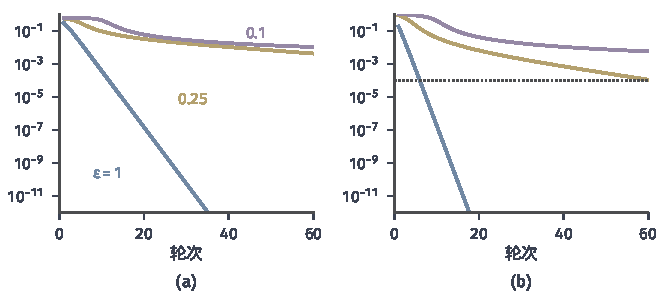
\includegraphics[width=112mm]{figures/07-probability/07-distribution-optimization/matplotlib/ot-sinkhorn-convergence/figure.pdf}
 \caption{全章例子上对数域Sinkhorn迭代的收敛，纵轴为对数刻度：$\varepsilon=1$（蓝）、$0.25$（黄）、$0.1$（紫）。(a)行残差$\rho^{(t)}$。(b)修正后可行方案的原对偶差$\Delta^{(t)}$，深灰点线为容差$10^{-4}$。}
 \label{fig:ot-sinkhorn-convergence}
\end{BookInlineFigure}

\paragraph{三种误差}
用熵正则化近似一个分布之间的运输问题时，最终结果与真正的$\operatorname{OT}_c(\mu,\nu)$之间有三种误差，应分别记录。离散化误差来自把$\mu,\nu$换成有限网格或有限样本上的分布，它取决于网格尺度或样本数。正则化偏差由式~\eqref{eq:ot-entropic-bias}控制，随$\varepsilon$线性减小。迭代误差由停止判据式~\eqref{eq:ot-sinkhorn-stop}控制。减小$\varepsilon$能降低偏差，却使迭代变慢、对数域计算变得必要；三者要在同一预算下权衡，不能只报告其中一项。若最终需要的是原问题的运输成本，还要报告$\langle\bm{C},\tilde{\bm{\pi}}\rangle$而不是正则化目标值。

\section{分布插值}
\label{sec:ot-interpolation}

给定两个分布$\mu_0,\mu_1$，怎样在它们之间连一条路径$\mu_t$，$0\leq t\leq1$？最直接的是混合$(1-t)\mu_0+t\mu_1$：质量不动，只是把权重从一个分布渐渐挪到另一个。取$\mu_0=\delta_0$，$\mu_1=\delta_1$，混合路径在中途是$\tfrac12\delta_0+\tfrac12\delta_1$，一半质量在$0$、一半在$1$，中间位置$\tfrac12$上什么也没有。若把分布想成一堆土，更自然的中途状态是“土堆搬到了一半的路上”，即$\delta_{1/2}$。最优运输给出这种路径：沿最优耦合把每份质量匀速推向它的目的地。

\begin{definition}[位移插值]
\label{def:ot-displacement}
设$\mu_0,\mu_1$是$\mathbb{R}^{d}$上具有有限二阶矩的分布，$\pi$是它们在平方欧氏成本下的一个最优耦合。对$0\leq t\leq1$，令$e_t(x,y)=(1-t)x+ty$，称
\begin{equation}
 \mu_t=(e_t)_\#\pi
 \label{eq:ot-displacement}
\end{equation}
为沿$\pi$的\term{位移插值}（displacement interpolation）。
\end{definition}

用随机向量说，取$(X,Y)\sim\pi$，$\mu_t$就是$(1-t)X+tY$的分布：每份质量从$X$出发，沿直线匀速走到$Y$，$t$时刻走完全程的$t$。$e_0,e_1$是两个坐标投影，所以端点正是$\mu_0,\mu_1$。$(1-t)x+ty$的平方范数不超过$2\lVert x\rVert_2^{2}+2\lVert y\rVert_2^{2}$，所以$\mu_t$也有有限二阶矩。

\begin{theorem}[位移插值是常速测地线]
\label{thm:ot-geodesic}
在定义~\ref{def:ot-displacement}的条件下，对一切$0\leq s\leq t\leq1$，
\begin{equation}
 W_2(\mu_s,\mu_t)=(t-s)\,W_2(\mu_0,\mu_1).
 \label{eq:ot-geodesic}
\end{equation}
\end{theorem}

\begin{proof}
记$W=W_2(\mu_0,\mu_1)$，$(X,Y)\sim\pi$。$\bigl((1-s)X+sY,\ (1-t)X+tY\bigr)$是$\mu_s$与$\mu_t$的一个耦合，两分量之差为$(t-s)(Y-X)$，所以
\[
 W_2^{2}(\mu_s,\mu_t)\leq(t-s)^{2}\,\mathbb{E}\lVert X-Y\rVert_2^{2}=(t-s)^{2}W^{2} .
\]
同样得到$W_2(\mu_0,\mu_s)\leq sW$，$W_2(\mu_t,\mu_1)\leq(1-t)W$。由$W_2$的三角不等式（第~\ref{chap:distribution-comparison}章），
\[
 \begin{aligned}
 W&\leq W_2(\mu_0,\mu_s)+W_2(\mu_s,\mu_t)+W_2(\mu_t,\mu_1)\\
 &\leq sW+(t-s)W+(1-t)W=W .
 \end{aligned}
\]
两端相等，中间每个不等号都必须取等，于是式~\eqref{eq:ot-geodesic}成立。
\end{proof}

式~\eqref{eq:ot-geodesic}说的是：$t\mapsto\mu_t$在度量$W_2$下走的是一条最短路，并且匀速，称为常速\term{测地线}（geodesic）。沿路径任意两点之间的距离恰好等于参数之差乘以全长，路径上不存在任何绕路。

\paragraph{两个点质量}
$\delta_0$与$\delta_1$之间只有一个耦合，位移插值是$\mu_t=\delta_t$，$W_2(\mu_s,\mu_t)=t-s$。混合路径$\nu_t=(1-t)\delta_0+t\delta_1$完全不同。$\nu_s$与$\nu_t$都在$\{0,1\}$上，它们在点$1$处的质量相差$t-s$，任何耦合至少要让这么多质量在$0$与$1$之间移动距离$1$；把恰好$t-s$的质量从$0$搬到$1$就做到了，所以
\[
 W_2(\nu_s,\nu_t)=\sqrt{t-s} .
\]
它不与$t-s$成正比。把$[0,1]$等分成$n$段，混合路径各段的$W_2$长度之和是$n\cdot\sqrt{1/n}=\sqrt{n}\to\infty$：按位置度量，混合路径根本不是一条有限长的路。图~\ref{fig:ot-point-interp}(a)对比了两种中途状态。

\begin{BookInlineFigure}
 \centering
 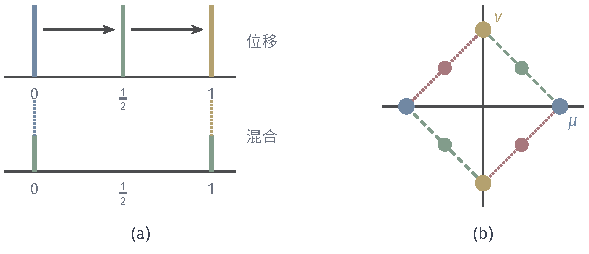
\includegraphics[width=108mm]{figures/07-probability/07-distribution-optimization/tikz/ot-point-interp/figure.pdf}
 \caption{位移插值与混合。(a)$\delta_0$（蓝）与$\delta_1$（黄）在$t=\tfrac12$的中途状态：上行是位移插值$\delta_{1/2}$，下行是混合$\tfrac12\delta_0+\tfrac12\delta_1$，竖线高度表示质量。(b)$\mu=\tfrac12(\delta_{(1,0)}+\delta_{(-1,0)})$（蓝）与$\nu=\tfrac12(\delta_{(0,1)}+\delta_{(0,-1)})$（黄），任何耦合都最优；绿色与红色分别是两个不同最优耦合的中点。}
 \label{fig:ot-point-interp}
\end{BookInlineFigure}

\paragraph{全章例子}
逐格搬运是平方成本下唯一的最优方案。$t=\tfrac12$时，留在$0$与$2$的质量不动，从$0$搬往$1$的$0.3$走到$0.5$，从$1$搬往$2$的$0.3$走到$1.5$：
\[
 \mu_{1/2}=0.2\,\delta_0+0.3\,\delta_{0.5}+0.3\,\delta_{1.5}+0.2\,\delta_2 .
\]
它与两端的距离都是$\tfrac12W_2=\tfrac12\sqrt{0.6}\approx0.387$。同一时刻的混合是$0.35\,\delta_0+0.3\,\delta_1+0.35\,\delta_2$，仍只放在原来的三个位置上。

\paragraph{一维高斯分布}
$\mu_0=\mathcal{N}(m_0,\sigma_0^{2})$与$\mu_1=\mathcal{N}(m_1,\sigma_1^{2})$之间的最优映射是$T(x)=m_1+(\sigma_1/\sigma_0)(x-m_0)$。取$X\sim\mu_0$，
\[
 (1-t)X+tT(X)=(1-t)m_0+tm_1+\Bigl((1-t)+t\frac{\sigma_1}{\sigma_0}\Bigr)(X-m_0),
\]
所以
\begin{equation}
 \mu_t=\mathcal{N}\Bigl((1-t)m_0+tm_1,\ \bigl((1-t)\sigma_0+t\sigma_1\bigr)^{2}\Bigr).
 \label{eq:ot-gaussian-geodesic}
\end{equation}
均值与标准差都线性变化，路径上始终是单峰的高斯分布。混合路径在中途是双峰的。图~\ref{fig:ot-displacement}取$m_0=-2$，$\sigma_0=0.5$，$m_1=2$，$\sigma_1=1$，画出两条路径。

\begin{BookInlineFigure}
 \centering
 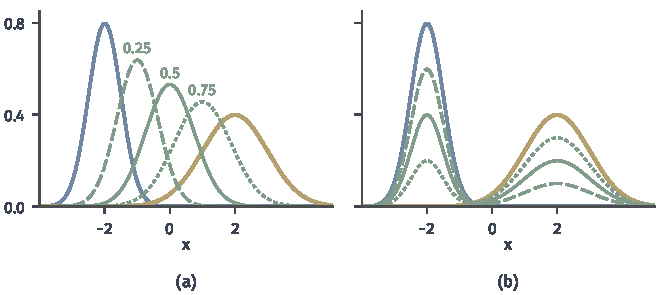
\includegraphics[width=112mm]{figures/07-probability/07-distribution-optimization/matplotlib/ot-displacement/figure.pdf}
 \caption{$\mathcal{N}(-2,0.5^{2})$（蓝）与$\mathcal{N}(2,1)$（黄）之间的两条路径，绿线是$t=0.25$（虚线）、$0.5$（实线）、$0.75$（点线）时的密度。(a)位移插值，密度整体平移并逐渐变宽。(b)混合，两个峰原地不动，只是高度此消彼长。}
 \label{fig:ot-displacement}
\end{BookInlineFigure}

\paragraph{插值不唯一}
定义~\ref{def:ot-displacement}依赖所选的最优耦合。最优耦合不唯一时，插值也不唯一。在$\mathbb{R}^{2}$中取
\[
 \mu=\tfrac12\bigl(\delta_{(1,0)}+\delta_{(-1,0)}\bigr),\qquad \nu=\tfrac12\bigl(\delta_{(0,1)}+\delta_{(0,-1)}\bigr).
\]
四个源—目标点对的平方距离都是$2$，所以每个耦合的成本都是$2$，全部最优。把$(1,0)$送到$(0,1)$、$(-1,0)$送到$(0,-1)$，中点落在$(\tfrac12,\tfrac12)$与$(-\tfrac12,-\tfrac12)$；交换目的地，中点落在另一条对角线上；独立耦合则在四个中点上各放$\tfrac14$。三者都是$\mu$与$\nu$之间的常速测地线在$t=\tfrac12$处的状态，见图~\ref{fig:ot-point-interp}(b)。

若$\mu_0$关于Lebesgue测度绝对连续，平方成本下的最优耦合唯一，并且由某个凸函数$\phi$的梯度给出：$\pi=(\mathrm{id},\nabla\phi)_\#\mu_0$。这时插值也唯一：
\[
 \mu_t=\bigl((1-t)\mathrm{id}+t\nabla\phi\bigr)_\#\mu_0 .
\]第~\ref{sec:ot-gaussian}节的对称正定线性映射就是$\phi$为二次函数的情形。一般情形的证明要用凸函数的几乎处处可微性，可查阅~\scite{math-villani2009transport}。

\section{Wasserstein重心}
\label{sec:ot-barycenter}

上一节在两个分布之间取中途状态。有多个分布时，能否找一个分布共同代表它们？对点$x_1,\dots,x_K\in\mathbb{R}^{d}$与权重$\lambda_k$，加权平均$\bar{x}=\sum_k\lambda_kx_k$是使$\sum_k\lambda_k\lVert y-x_k\rVert_2^{2}$最小的点。把点换成分布、把平方距离换成$W_2^{2}$，就得到分布的“平均”。

\begin{definition}[Wasserstein重心]
\label{def:ot-barycenter}
设$\mu_1,\dots,\mu_K$是$\mathbb{R}^{d}$上具有有限二阶矩的分布，权重$\lambda_k\geq0$，$\sum_k\lambda_k=1$。在有限二阶矩的分布$\nu$中最小化
\begin{equation}
 \Psi(\nu)=\sum_{k=1}^{K}\lambda_kW_2^{2}(\nu,\mu_k),
 \label{eq:ot-barycenter}
\end{equation}
最小点称为$\mu_1,\dots,\mu_K$关于这组权重的\term{Wasserstein重心}（Wasserstein barycenter）。
\end{definition}

它与混合分布$\sum_k\lambda_k\mu_k$是两回事。混合把各分布的质量按权重叠在一起，质量都留在原处；重心则把质量搬到“平均位置”上。

\paragraph{点质量的重心}
取$\mu_k=\delta_{x_k}$。任何$\nu$与点质量只有一个耦合，即$\nu\otimes\delta_{x_k}$，所以
\[
 W_2^{2}(\nu,\delta_{x_k})=\int\lVert y-x_k\rVert_2^{2}\,\nu(\mathrm{d}y).
\]对每个$y$有恒等式
\[
 \sum_k\lambda_k\lVert y-x_k\rVert_2^{2}=\lVert y-\bar{x}\rVert_2^{2}+\sum_k\lambda_k\lVert x_k-\bar{x}\rVert_2^{2},
\]
因为交叉项$2\sum_k\lambda_k\langle y-\bar{x},\bar{x}-x_k\rangle$中$\sum_k\lambda_k(\bar{x}-x_k)=0$。对$\nu$积分，
\[
 \Psi(\nu)=\int\lVert y-\bar{x}\rVert_2^{2}\,\nu(\mathrm{d}y)+\sum_k\lambda_k\lVert x_k-\bar{x}\rVert_2^{2},
\]
第一项在且仅在$\nu=\delta_{\bar{x}}$时为零。所以点质量的重心唯一，是$\delta_{\bar{x}}$，正是点的加权平均；混合分布$\sum_k\lambda_k\delta_{x_k}$则在每个$x_k$上各放一份质量。

\paragraph{两个分布的重心}
$K=2$、权重$(1-t,t)$时，位移插值$\mu_t$是重心。记$W=W_2(\mu_0,\mu_1)$，任取$\nu$，令$\alpha=W_2(\nu,\mu_0)$，$\beta=W_2(\nu,\mu_1)$，由三角不等式$\alpha+\beta\geq W$。直接展开可以验证
\[
 (1-t)\alpha^{2}+t\beta^{2}-t(1-t)(\alpha+\beta)^{2}=\bigl((1-t)\alpha-t\beta\bigr)^{2}\geq0 ,
\]
所以$\Psi(\nu)\geq t(1-t)W^{2}$。由定理~\ref{thm:ot-geodesic}，$\mu_t$满足$\alpha=tW$，$\beta=(1-t)W$，代入得
\[
 \Psi(\mu_t)=(1-t)t^{2}W^{2}+t(1-t)^{2}W^{2}=t(1-t)W^{2},
\]
达到下界。

\paragraph{实数轴上的重心}
一维时，由定理~\ref{thm:ot-one-dimensional}，$W_2^{2}$是分位数函数之差的平方积分，重心问题化为分位数函数的最小二乘。

\begin{theorem}[一维重心]
\label{thm:ot-barycenter-1d}
设$\mu_1,\dots,\mu_K$是实数轴上具有有限二阶矩的分布，分位数函数为$F_k^{-1}$。则重心唯一，它的分位数函数是
\begin{equation}
 \bar{q}(u)=\sum_{k=1}^{K}\lambda_kF_k^{-1}(u),\qquad0<u<1 .
 \label{eq:ot-barycenter-1d}
\end{equation}
\end{theorem}

\begin{proof}
任取有限二阶矩的分布$\nu$，分位数函数为$G^{-1}$。由式~\eqref{eq:ot-quantile-formula}与点质量情形中的同一恒等式（逐个$u$使用），
\[
 \Psi(\nu)=\int_0^{1}\bigl(G^{-1}(u)-\bar{q}(u)\bigr)^{2}\,\mathrm{d}u+\sum_k\lambda_k\int_0^{1}\bigl(F_k^{-1}(u)-\bar{q}(u)\bigr)^{2}\,\mathrm{d}u .
\]
第二项与$\nu$无关。$\bar{q}$是单调不减、左连续函数的非负组合，仍单调不减且左连续；由各$F_k^{-1}$平方可积，它也平方可积。令$\bar{\nu}$为$\bar{q}(U)$的分布，$U\sim\operatorname{Unif}(0,1)$，由单调性与左连续性可以验证$\bar{\nu}$的分位数函数就是$\bar{q}$，并且$\bar{\nu}$有有限二阶矩。于是$\bar{\nu}$使第一项为零，是重心。反过来，任何重心都使第一项为零，$G^{-1}=\bar{q}$几乎处处成立；两个左连续单调函数几乎处处相等就处处相等，所以重心就是$\bar{\nu}$。
\end{proof}

对一维高斯分布$\mu_k=\mathcal{N}(m_k,\sigma_k^{2})$，$F_k^{-1}(u)=m_k+\sigma_k\Phi^{-1}(u)$，其中$\Phi$是标准高斯分布函数，于是重心是
\[
 \mathcal{N}\Bigl(\sum_k\lambda_km_k,\ \bigl(\textstyle\sum_k\lambda_k\sigma_k\bigr)^{2}\Bigr):
\]
均值平均，标准差也平均。图~\ref{fig:ot-barycenter}取三个形状不同的分布，$\mathcal{N}(-3,0.5^{2})$、$\operatorname{Unif}(-1,1)$与$\mathcal{N}(3.5,0.8^{2})$，权重各$\tfrac13$。重心的分位数函数是
\[
 \bar{q}(u)=\tfrac13\bigl(-0.5+1.3\,\Phi^{-1}(u)+2u\bigr),
\]
均值为$\tfrac16$，形状介于高斯与均匀之间，是一个单峰分布；混合分布则保留三个分开的峰。

\begin{BookInlineFigure}
 \centering
 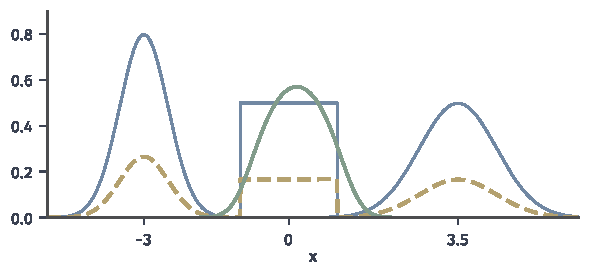
\includegraphics[width=100mm]{figures/07-probability/07-distribution-optimization/matplotlib/ot-barycenter/figure.pdf}
 \caption{三个分布（蓝）：$\mathcal{N}(-3,0.5^{2})$、$\operatorname{Unif}(-1,1)$、$\mathcal{N}(3.5,0.8^{2})$，权重各$\tfrac13$。绿线是Wasserstein重心的密度，由平均分位数函数式~\eqref{eq:ot-barycenter-1d}数值求得；黄色虚线是混合分布的密度。}
 \label{fig:ot-barycenter}
\end{BookInlineFigure}

\paragraph{存在与唯一}
一般维数中没有分位数可用，但存在性可以沿用第~\ref{sec:ot-existence}节的紧性论证。

\begin{theorem}[重心的存在]
\label{thm:ot-barycenter-existence}
在定义~\ref{def:ot-barycenter}的条件下，重心存在。
\end{theorem}

\begin{proof}
记$V=\inf_\nu\Psi(\nu)$，取$\nu=\mu_1$知$V<\infty$。取有限二阶矩的分布列$\nu_l$，使$\Psi(\nu_l)\to V$。

\emph{二阶矩一致有界。}取$\lambda_{k_0}>0$。$\lVert y\rVert_2^{2}$不超过$2\lVert y-x\rVert_2^{2}+2\lVert x\rVert_2^{2}$，在$\nu_l$与$\mu_{k_0}$的最优耦合下取期望，
\[
 \int\lVert y\rVert_2^{2}\,\nu_l(\mathrm{d}y)\leq\frac{2\Psi(\nu_l)}{\lambda_{k_0}}+2\int\lVert x\rVert_2^{2}\,\mu_{k_0}(\mathrm{d}x),
\]
右边对$l$有界，记为$M$。由第~\ref{chap:weak-convergence-of-distributions}章的矩条件，$\{\nu_l\}$胎紧，有子列（仍记为$\nu_l$）弱收敛到某个$\nu$。对每个$R>0$，$\min(\lVert y\rVert_2^{2},R)$有界连续，其积分在极限中不超过$M$；令$R\to\infty$，$\nu$的二阶矩不超过$M$。

\emph{距离下半连续。}固定$k$，取子列使$W_2^{2}(\nu_l,\mu_k)$趋于它的下极限，取最优耦合$\pi_l\in\Pi(\nu_l,\mu_k)$。$\{\nu_l\}$与$\mu_k$都胎紧，按引理~\ref{lem:ot-coupling-compact}的证明，$\{\pi_l\}$胎紧，再取子列使$\pi_l\xrightarrow{\mathrm{w}}\pi$。对有界连续的$h$，
\[
 \int h(x)\,\pi(\mathrm{d}x,\mathrm{d}y)=\lim_{l\to\infty}\int h\,\mathrm{d}\nu_l=\int h\,\mathrm{d}\nu ,
\]
所以$\pi$的第一边缘是$\nu$；每个$\pi_l$的第二边缘都是$\mu_k$，同样的论证说明$\pi$的第二边缘也是$\mu_k$。由引理~\ref{lem:ot-cost-lsc}，
\[
 W_2^{2}(\nu,\mu_k)\leq\int\lVert x-y\rVert_2^{2}\,\mathrm{d}\pi\leq\liminf_{l\to\infty}W_2^{2}(\nu_l,\mu_k).
\]
对$k$加权求和，下极限之和不超过和的下极限，于是$\Psi(\nu)\leq\liminf_l\Psi(\nu_l)=V$。
\end{proof}

唯一性需要额外条件。若某个权重为正的$\mu_k$关于Lebesgue测度绝对连续，重心唯一。机制是：这时$\nu\mapsto W_2^{2}(\nu,\mu_k)$在分布的混合下严格凸，而$\Psi$的其余各项是凸的；严格凸性来自第~\ref{sec:ot-interpolation}节提到的最优耦合由凸函数梯度唯一给出，证明可查阅前面提到的Villani的专著。条件不能随意去掉。在第~\ref{sec:ot-interpolation}节的正方形例子中取权重$(\tfrac12,\tfrac12)$，两个分布都是点质量组成的，不绝对连续；三种不同的中途状态都满足$\alpha=\beta=\tfrac12W$，都使$\Psi$达到下界$\tfrac14W^{2}$，所以重心不唯一。一维情形是例外，定理~\ref{thm:ot-barycenter-1d}对任何有限二阶矩的分布都给出唯一性。

\section{本章小结}
\label{sec:ot-summary}

本章从一个问题出发：两个边缘分布固定，怎样把一个搬成另一个最省。可行方案是全部耦合，它们构成一个凸集；在有限情形是运输多面体，在一般情形靠固定边缘带来的胎紧性获得紧性。成本非负下半连续时最优耦合存在；去掉下半连续，极小化序列可能在极限处跳高。存在的是最优耦合，不是最优映射：映射要求质量不可拆分，可能连可行解都没有，或者下确界取不到。

最优性的证据来自对偶。满足$\varphi(x)+\psi(y)\leq c(x,y)$的一对势给出一切耦合成本的公共下界，原对偶差等于耦合下松弛量的积分，所以质量只落在零松弛处的耦合就是最优的。有限情形的强对偶由线性规划得到，紧致空间上的连续成本可以由有限问题逼近得到；原问题达到、无对偶间隙与最优势存在是三个不同的结论，需要分别核对条件。

具体结构决定怎样求解。表~\ref{tab:ot-summary}汇总本章求解的几类问题。

\begin{table}[htbp]
 \centering
 \caption{本章求解的运输问题。高斯两行为平方成本，实数轴一行要求$p\geq1$与有限$p$阶矩；“映射”一列指最优方案是否由运输映射实现。}
 \label{tab:ot-summary}
 \begin{tabular}{lll}
  \toprule
  问题 & 最优方案 & 映射\\
  \midrule
  实数轴，$\lvert x-y\rvert^{p}$ & 分位数耦合 & 源无原子时是\\
  有限支持 & 线性规划的顶点 & 一般不是\\
  高斯，$\bm{\Sigma}_1$正定 & 对称正定仿射映射 & 是\\
  高斯，$\bm{\Sigma}_1$奇异 & 按支撑子空间分析 & 可能不是\\
  熵正则化 & 行列缩放式~\eqref{eq:ot-scaling-form} & 不是\\
  \bottomrule
 \end{tabular}
\end{table}

一维问题证明了第~\ref{chap:distribution-comparison}章提到的关系：$W_1$等于两条分布函数之间的面积，$W_p^{p}$等于分位数函数之差的$p$次方积分。全章例子中，逐格搬运同时被对偶势、分位数耦合证实为平方成本下唯一的最优方案，成本$0.6$。熵正则化把运输问题变成严格凸的光滑问题，解具有行列缩放形式，Sinkhorn迭代交替满足行和与列和；正则化偏差不超过$\varepsilon$乘以最优方案与独立方案之间的KL散度，迭代误差由修正可行方案后的原对偶差控制，两者与离散化误差要分别报告。

最后两节用最优耦合构造新的分布。位移插值把每份质量沿直线匀速推向目的地，是$W_2$下的常速测地线；混合路径则只调整权重，在$W_2$下甚至不是有限长的路径。Wasserstein重心推广了点的加权平均，在有限二阶矩下存在；一维时就是分位数函数的加权平均，高维时唯一性需要某个正权重分布绝对连续。最优耦合不唯一时，插值与重心都不唯一。

本章始终在成本、矩条件、映射可行性与数值误差的范围内下结论：有限$p$阶矩保证成本有限，下半连续保证最优耦合存在，严格凸成本与绝对连续的源分布才带来唯一性与映射，正则化与迭代给出的是带有可计算误差界的近似。$W_p$作为距离的性质及其与弱收敛的关系，分别见第~\ref{chap:distribution-comparison}章与第~\ref{chap:weak-convergence-of-distributions}章。

